\documentclass[
  bibliography=totoc,     % Literatur im Inhaltsverzeichnis
  captions=tableheading,  % Tabellenüberschriften
  titlepage=firstiscover, % Titelseite ist Deckblatt
]{scrartcl}

\usepackage[ngerman]{babel} 
\usepackage[utf8]{inputenc}
\usepackage[T1]{fontenc} 
\usepackage{lmodern}
\usepackage{setspace}
\usepackage{wrapfig} %Für Bilder
\usepackage{xcolor} %Farbe

%\usepackage{scrpage2}

\usepackage{amssymb} % Mathe Symbole
\usepackage{amsmath} % Mathe
\usepackage{mathtools} % Erweiterungen für amsmath
\usepackage{esvect} %Für vektoren

\usepackage{setspace} % Fuer eine Liste mit Abk.
\usepackage{listings} % Um Code schoener aussehen zu lassen

% Zahlen und Einheiten
\usepackage[
  locale=DE,                   % deutsche Einstellungen
  separate-uncertainty=true,   % immer Fehler mit \pm
  per-mode=symbol-or-fraction, % / in inline math, fraction in display math
]{siunitx}

% chemische Formeln
\usepackage[
  version=4,
  math-greek=default, % ┐ mit unicode-math zusammenarbeiten
  text-greek=default, % ┘
]{mhchem}

% richtige Anführungszeichen
\usepackage[autostyle]{csquotes}

% schöne Brüche im Text
\usepackage{xfrac}

% Standardplatzierung für Floats einstellen
\usepackage{float}
\floatplacement{figure}{htbp}
\floatplacement{table}{htbp}


%keine Floats in anderen Sectionen
\usepackage{placeins}

\let\Oldsection\section
\renewcommand{\section}{\FloatBarrier\Oldsection}

\let\Oldsubsection\subsection
\renewcommand{\subsection}{\FloatBarrier\Oldsubsection}

\let\Oldsubsubsection\subsubsection
\renewcommand{\subsubsection}{\FloatBarrier\Oldsubsubsection}

% Seite drehen für breite Tabellen: landscape Umgebung
\usepackage{pdflscape}

% Captions schöner machen.
\usepackage[
  labelfont=bf,        % Tabelle x: Abbildung y: ist jetzt fett
  font=small,          % Schrift etwas kleiner als Dokument
  width=0.9\textwidth, % maximale Breite einer Caption schmaler
]{caption}
% subfigure, subtable, subref
\usepackage{subcaption}

% Grafiken können eingebunden werden
\usepackage{graphicx}
% größere Variation von Dateinamen möglich
\usepackage{grffile}

% schöne Tabellen
\usepackage{booktabs}

% Verbesserungen am Schriftbild (scheint zu Fehlern zu führen)
%\usepackage{microtype}

% Literaturverzeichnis
\usepackage[
  backend=biber,
]{biblatex}
% Quellendatenbank
\addbibresource{lit.bib}
\addbibresource{programme.bib}

% Hyperlinks im Dokument
\usepackage[
  unicode,        % Unicode in PDF-Attributen erlauben
  pdfusetitle,    % Titel, Autoren und Datum als PDF-Attribute
  pdfcreator={},  % ┐ PDF-Attribute säubern
  pdfproducer={}, % ┘
]{hyperref}

% erweiterte Bookmarks im PDF
\usepackage{bookmark}

%erweiterte Aufzählungen
\usepackage{paralist}

% Trennung von Wörtern mit Strichen
\usepackage[shortcuts]{extdash}

\author{%
  David Rolf%
  \texorpdfstring{%
    \\%
    \href{mailto:david.rolf@tu-dortmund.de}{david.rolf@tu-dortmund.de}
  }{}%
  \texorpdfstring{\and}{, }%
  Jonah Blank%
  \texorpdfstring{%
    \\%
    \href{mailto:jonah.blank@tu-dortmund.de}{jonah.blank@tu-dortmund.de}
  }{}%
}
%\publishers{TU Dortmund – Fakultät Physik}

% Ableitungen mit \diff
\newcommand{\diff}{\mathop{}\!\mathrm{d}}

% mache . zu einem aktiven Zeichen im Mathemodus 
\mathcode`\.="8000 
% Dann kommt die Umdefinition des Dezimalpunktes 
\begingroup\lccode`~=`. 
  \lowercase{\endgroup\def~}#1{\mathrm{#1}} 
\usepackage{rotating}
\subject{V14}
\title{\texorpdfstring{Tomographie mit Gamma-Strahlen}{}}
\date{
\begin{center}
	 Durchführung: 09.12.2019 \hspace{3em} Abgabe: 12.12.2019\\
	 \begin{figure}
	 \centering
	 \includegraphics[scale=0.2]{content/images/tu.jpg}
	 \end{figure}
	 Fakultät Physik
\end{center}
}

\begin{document}
	\maketitle
	\newpage
	\tableofcontents
	\newpage
	
\section{Zielsetzung}
\label{sec:Zielsetzung}

Ziel des Versuchs ist die Plateau-Steigung und die Totzeit eines Geiger-Müller-Zählrohres, sowie die pro Teilchen freigesetzte Ladungsmenge zu bestimmen. Darüber hinaus wird die Erholungszeit gemessen.

	\section{Theorie}
\label{sec:Theorie}
%Bei einer Besetzungsinversion wird die induzierte Abkehr von der thermischen Besetzungswahrscheinlichkeit der Energieniveaus eines Atoms herbeigeführt.
%Um dies zu verstehen ist es zunächst nötig, die elektronische Struktur des hier untersuchten Elements Rubidium zu erläutern.

\subsection{Beschreibung der Energieniveaus in Rubidium}
\label{subsec:energieniveaus}

Bei Rubidium handelt es sich um ein Alkalimetall, das nur über ein ungepaartes Elektron in der fünften Schale verfügt, sodass nur dieses zu den Quantenzahlen der Elektronenhülle beiträgt.
Ohne Betrachtung von Korrekturen befindet es sich als Spin-1/2-Teilchen in dem Zustand mit $n=5$, $L=0$ und $M_L=0$. Dabei ist $n$ die Hauptquantenzahl, $L$ die Drehimpulsquantenzahl und $M_L$ die zu ihr gehörige magnetische Quantenzahl. \\
Die Zustände sind entartet. Diese Entartung kann durch die Feinstruktur, die Hyperfeinstruktur und den Zeeman-Effekt aufgehoben werden (vergleiche Abbildung \ref{fig:energieniveaus}).
%In niedrigster Ordnung verfügt das Niveau mit $L=1$ und $M_L=0,\pm1$ über die gleiche Energie wie der besetzte Zustand. Sie sind entartet.\\

\begin{figure}
  	\centering
  	\includegraphics[width=0.88\textwidth,keepaspectratio]{content/images/energieniveaus.png}
  	\caption{Energieniveaus in \ce{^{87}Rb} mit $I=3/2$ (nicht maßstäblich) \cite{alt}.}
  	\label{fig:energieniveaus}
\end{figure}

\subsubsection{Elektronenspin und Feinstruktur}
Der Gesamtdrehimpuls $\vec{J}$ einer Elektronenhülle eines Atoms setzt sich aus Bahndrehimpuls $\vec{L}$ und Spin $\vec{S}$ wie folgt zusammen:
\begin{equation*}
  \vec{J} = \vec{L} + \vec{S} \text{.}
\end{equation*}
Dies kommt durch die Spin-Bahn-Kopplung des Elektronenspins zustande.
Die Quantenzahlen $J$ und $M_J$ definieren nun statt $L$ und $M_L$ einen gegebenen Zustand, wobei $J$ von $\lvert L - S \rvert$ bis $\lvert L + S \rvert$ reicht. Zustände mit verschiedenem $J$ sind in dieser Feinstruktur nicht mehr energetisch entartet, während Zustände mit gleichem $J$ und verschiedenem $M_J$ ohne äußeres Magnetfeld energetisch entartet bleiben.

\subsubsection{Kernspin und Hyperfeinstruktur}
Die Niveaus werden in eine weitere Hyperfeinstruktur aufgespalten, wenn die Spin-Spin-Kopplung des Kernspins an den Gesamtdrehimpuls der Elektronenhüllen berücksichtigt wird. Es ergibt sich für den Gesamtdrehimpuls $\vec{F}$ des Atoms:
\begin{equation*}
  \vec{F} = \vec{J} + \vec{I} \text{.}
\end{equation*}
Zu diesem gehört die Quantenzahl $F$, die Werte von $\lvert J - I \rvert$ bis $\lvert J + I \rvert$ annimmt, mit der magnetischen Quantenzahl $M_F$. 
%In Abbildung \ref{fig:energieniveaus} werden die Feinstrukturniveaus dementsprechend jeweils in zwei Niveaus aufgespalten, wobei wieder Zustände mit gleichem $F$ und verschiedenem $M_F$ ohne äußeres Magnetfeld energetisch entartet bleiben.\\

\subsubsection{Der Zeeman-Effekt}
Die Aufhebung der Entartung dieser Zustände durch ein Magnetfeld geschieht durch den sogenannten Zeeman-Effekt. Dieser spaltet einen $F$-Zustand wiederum in $2F$+1-Zustände auf. Die Energiedifferenz zweier benachbarter Zeeman-Niveaus beträgt
\begin{equation}
\Delta E_Z = g_F \mu_{\text{B}} B
\label{eqn:zeemanDifferenz}
\end{equation}
und ist somit proportional zur magnetischen Flussdichte $B$. Der Faktor $\mu_{\text{B}} = \frac{e \hbar}{2m_e}$ ist das Bohrsche Magneton.\\
Der Landé-Faktor des Gesamtdrehimpulses des Atoms $g_F$ ergibt sich aus Kopplungsdiagrammen der beteiligten Drehimpulse näherungsweise zu
\begin{equation}
g_F = g_J \frac{F(F+1)+J(J+1)-I(I+1)}{2F(F+1)}\,,
\label{eqn:g_F_Theorie}
\end{equation}
wobei der Landé-Faktor des Gesamtdrehimpulses des Elektrons $g_J$ gegeben ist durch:
\begin{equation}
g_J = \frac{3{,}0023J(J+1)+1{,}0023(S(S+1)-L(L+1))}{2J(J+1)}
\label{eqn:g_J_Theorie}
\end{equation}

\subsubsection{Abschätzung des quadratischen Zeeman-Effekts}
\label{subsec:quadratischerZeeman}

%Um Felder mittlerer Stärke zu betrachten, werden weitere Ordnungen der Störungstheorie bei der Berechnung des Zeeman-Effekts berücksichtigt. In niedrigster Ordnung ist dies dann der quadratische Zeeman-Effekt, sodass die Energiedifferenz aus Gleichung \eqref{eqn:zeemanDifferenz} zu
Im Falle großer Magnetfelder entstehen aufgrund der Wechselwirkungen des Spins mit dem Bahndrehimpuls und der Wechselwirkung der magnetischen Momente weitere Effekte, welche bei der Zeemann-Aufspaltung berücksichtigt werden müssen. In niedrigster Ordnung Störungstheorie ist dies dann der quadratische Zeeman-Effekt.
Es ergibt sich für die Zeemann-Aufspaltung als Erweiterung von Formel \eqref{eqn:zeemanDifferenz}:
\begin{equation}
\Delta E_Z = g_F \, \mu_{\text{B}} B + g_F^2 \, \mu_{\text{B}}^2 B^2 \frac{1-2M_F}{\Delta E_{\text{Hy}}},
\label{eqn:zeemanDifferenzQuadratisch}
\end{equation}
wobei $E_\text{Hy}$ die Hyperfeinstrukturaufspaltung zwischen den Niveaus zwischen $F$ und $F+1$ bezeichnet.


\subsection{Optisches Pumpen}
\label{subsec:prinzipOptischesPumpen} 

\subsubsection{Prinzip des optischen Pumpens}

%Es ist üblich, die Feinstrukturniveaus als Termsymbole ${}^{2S+1}L_J$ mit der Multiplizität $2S+1$ und dem Kennbuchstaben $L$ für den elektronischen Drehimpuls zu schreiben, wobei für $L=0$ ein S und für $L=1$ ein P geschrieben wird.
Beim optischen Pumpen werden die Niveaus entegegen der thermischen Verteilung besetzt.
%Es ist also möglich, die Verteilung der äußeren Hüllenelektronen zu invertieren.
Für das optische Pumpen an Rubidium ist die Aufspaltung der Hyperfeinstrukturniveaus durch den Zeeman-Effekt nötig. Die Besetzung folgt dann näherungsweise einer thermischen Boltzmann-Verteilung, sodass die Elektronen größtenteils im Grundzustand mit niedrigstem $m_F$ angereichert sind.\\
In diesem Versuch wird rechtszirkular polarisiertes Licht der Frequenz des $D_1$-Übergangs eingestrahlt. Übergänge, die durch Absorption dieser Photonen entstehen (stimulierte Emission) gehorchen der Auswahlregel $\Delta M_F=+1$, während die spontane Emission keine bestimmten Übergänge bevorzugt. Dadurch werden die unteren Niveaus entleert und der S-Zustand mit $F=2$, $M_F=2$ angereichert. Es wird eine Besetzungsinversion herbeigeführt. Eine schematische Darstellung der Übergänge findet sich in Abbildung \ref{fig:pumpschema}.

\begin{figure}
	\centering
	\includegraphics[width=0.96\textwidth,keepaspectratio]{content/images/pumpschema.png}
	\caption{Pumpschema für \ce{^{87}Rb} ($I=3/2$) zur Herstellung einer Besetzungsinversion \cite{caltech}.}
    \label{fig:pumpschema}
\end{figure}

\noindent Ein geeignetes Maß für die Besetzungsinversion stellt die Transparenz der Dampfzelle gegenüber dem einstrahlenden $D_1$-Licht dar. Diese wird mit einer ansteigenden Exponentialfunktion parametrisiert, welche sich bei vollständiger Inversion sättigt.\\

\subsubsection{Einfluss eines hochfrequenten magnetischen Feldes}
Optischen Pumpen wird oft als spektroskopisches Verfahren eingesetzt, um die aufgespaltenen Energieniveaus mit hoher Genauigkeit zu vermessen. Dieses Messverfahren bedient sich eines zweiten, hochfrequenten magnetischen Feldes (RF-Feld), welches stimulierte Emission aus dem angereicherten Niveau heraus anregt. Für die dafür benötigte Flussdichte $B_m$ gilt die Beziehung
\begin{equation}
h f = g_F \, \mu_{\text{B}} B_m \Delta M_F \implies B_m = \frac{4 \pi m_e}{e g_F} f
\label{eqn:B_M_Theorie}
\end{equation}
%sodass ein linearer Zusammenhang zu der Frequenz des Feldes besteht.
Da mit der stimulierten Emission eine Entleerung des zuvor angereicherten Niveaus verbunden wird, ist das Erreichen der Feldstärke $B_m$ mit einer deutlichen Abnahme der Transparenz des Gases verbunden. %, weil der konkurrierende Prozess der Besetzungsinversion durch optisches Pumpen wieder aufnehmen kann (vergleiche Abbildung \ref{fig:transparenz}).\\
Um 0 herum sinkt die Transparenz ebenfalls deutlich ab, da es ohne Äußeres Magnetfeld nicht zu einer Zeeman-Aufspaltung kommen kann (vergleiche Abbildung \ref{fig:transparenz}). %Experimentell wird dies ausgenutzt, um den Einfluss des Erdmagnetfelds zu minimieren.

\begin{figure}
    \centering
    \includegraphics[width=\textwidth-120pt,keepaspectratio]{content/images/transparenz.png}
  	\caption{Transparenz der Dampfzelle in Abhängigkeit eines äußeren Magnetfelds \cite{V21}.}
    \label{fig:transparenz}
\end{figure}

\newpage
\subsubsection{Transiente Effekte}
\label{subsec:transient}

Beim schnellen Ein- und Ausschalten des RF-Feldes zeigt sich, dass der Spin $\vec{F}$ im rotierenden Koordinatensystem um die Achse des RF-Feldes präzediert, wenn das statische Magnetfeld resonant eingestellt ist. Die Lamor-Frequenz beträgt dabei $\gamma B_{\text{RF}}$ mit dem gyromagnetischen Verhältnis 
\[
\gamma = g_F \frac{\mu_{\text{B}}}{\hbar},
\]
sodass die Periodendauer der sogenannten Rabi-Oszillation 
\[
T=\frac{1}{(\gamma B_\text{RF})}
\]
amplitudenabhängig ist.
Es gilt:
\begin{equation}
\frac{T_{87}}{T_{85}} = \frac{\gamma_{85}}{\gamma_{87}}
\label{eqn:transient}
\end{equation}

\subsection{Helmholtzspule}

Helmholtzspulen erzeugen in ihrem inneren ein nahezu homogenes Magnetfeld $B$. Dieses wird berechnet über:
\begin{equation}
B = \mu_0\frac{8}{\sqrt{125}}\frac{IN}{R},
\label{eq:helmholtz}
\end{equation}
mit der magnetischen Feldkonstanten $mu_0$, der Windungszahl $N$ und dem Radius $R$ der Spule, sowie dem angelegten Strom $I$.
	\section{Aufbau}
\label{sec:Aufbau}

In Abbildung \ref{fig:Aufbau} ist der experimentelle Aufbau des Versuchs zu sehen.
Der verwendete Halbleiter GaAs ist durchlässig für infrarotes Licht.
Als Lichtquelle wird deshalb eine Halogenlampe verwendet.
Nach der Bündelung des Lichtes über eine Sammellinse, wird es über ein sich drehendes Rad, den Lichtzerhacker, in Lichtpulse aufgeteilt.
Der Polarisator teilt den Lichtstrahl durch unterschiedliche Brechungsindizes der Komponenten im Polarisatormedium in einen ordentlichen s- und einen außerordentlich p-polarisierten Teil. Der s-Anteil wird dabei total reflektiert, während der p-Anteil transmittiert wird.
Das nun linear polarisierte Licht fällt auf eine Probe aus Galliumarsenid, welche sich im Feld eines Elektromagneten befindet. Über einen Interferenzfilter wird eine bestimmte Wellenlänge herausgefiltert und der Lichtstrahl trifft auf einen weiteren als Analysator dienenden Polarisator. Aus diesem treten zwei zueinander orthogonal polarisierte Strahlen aus, welche an zwei Photowiderstände Spannungen erzeugen.
Diese werden in einen Differenzverstärker gegeben, der an ein Oszilloskop angeschlossen ist. Die Frequenz des Differenzverstärkers ist zur Rauschunterdrückung auf die des Lichzerhackers abgestimmt und die ausgehende Spannung ist genau dann $0$, wenn die beiden vermessenen identisch sind.

\begin{figure}
\centering
\includegraphics[width=0.9\textwidth]{content/images/aufbau.png}
\caption{Schematischer Aufbau zur Untersuchung der Faraday-Rotation.\cite{V46}}
\label{fig:Aufbau}
\end{figure}
	\section{Durchführung}
\label{sec:Durchführung}

Zur Entgasung des Rezipienten wird dieser bei laufender Turbopumpe mit einem Heißluftföhn erhitzt um mögliche adsorbierte Wasserdampfrückstände zu beseitigen.

\subsection{Die Drehschieberpumpe}

Zur Messung der p(t)-Kurve der Drehschieberpumpe wird mit einem Belüftungsventil der Druck im Inneren des Rezipienten auf Normaldruck erhöht. Bei laufendem Pumpenbetrieb wird das Ventil wieder geschlossen und mit dem Pirani-Vakuummeter der Druck in Abhängigkeit von der Zeit gemessen.
Die Messung wird fünf Mal durchgeführt und der Enddruck $p_.E$ bestimmt.\newline
Zur Leckratenmessung wird ein Nadelventil angebracht und über dieses ein Gleichgewichtsdruck $p_.g$ im $\SI{1}{\milli\bar}$-Bereich eingestellt. Die Drehschieberpumpe wird über ein Ventil abgeschiebert und der Druckanstieg in Abhängigkeit von der Zeit am Pirani-Vakuummeter abgelesen.
Die Messung wird für vier verschiedene $p_.g$ jeweils drei Mal durchgeführt.

\subsection{Turbomolekularpumpe}

Nach Erzeugen des Vorvakuums durch die Drehschieberpumpe wird die Turbopumpe bis zur vollen Drehzahl von $\SI{1350}{\hertz}$ hochgefahren.
Zur Bestimmung der p(t)-Kurve wird bei laufender Pumpe, mit einem Nadelventil ein Druck von $p_.0=\SI{5e-3}{\milli\bar}$ eingestellt und nach schließen des Ventils auf dem Glühkathoden-Vakuummeter der Druckabfall in abhängig von der Zeit abgelesen. Die Messung wird fünf Mal durchgeführt.\newline
Für die Leckratenmessung wird mit dem Nadelventil ein Gleichgewichtsdruck zwischen $5$ und $\SI{20e-5}{\milli\bar}$ eingestellt und nach Abschiebern der Pumpe der Druckanstieg in Abhängigkeit von der Zeit vom Glühkathoden-Vakuummeter abgelesen. Um Schäden am Glühkathoden-Vakuummeter zu vermeiden, wird dieses am Ende der Messung rechtzeitig ausgeschaltet und am weniger empfindlichen Kaltkathoden-Vakuummeter abgelesen, wann wieder ein ausreichend gutes Vakuum erreicht ist. Die Messung wird für 4 verschiedene Gleichgewichtsdrücke je drei Mal durchgeführt.


%☺☻☺
% ♥
	%\newpage
	\section{Auswertung}
\label{sec:Auswertung}

Die Graphen werden sowohl mit Matplotlib \cite{matplotlib} als auch NumPy \cite{numpy} erstellt. Die Fehlerrechnung wird mithilfe von Uncertainties \cite{uncertainties} durchgeführt.

\subsection{Modellierung: Teilchen im Potentialtopf}

In Abbildung \ref{fig:Uebersicht} ist das Übersichtsspektrum für eine $\SI{600}{\milli\meter}$-Röhre und in Abbildung \ref{fig:150} das einer $\SI{150}{\milli\meter}$-Röhre zu sehen.
Eine zweite Messung des Spektrums letzterer, liefert abgesehen von geringen Abweichungen in der Amplitude dasselbe Spektrum.
Beispielhaft sind die Parameter des 1. Peaks der beiden Messungen in Tabelle \ref{tab:param} zu sehen.

\begin{figure}
\centering
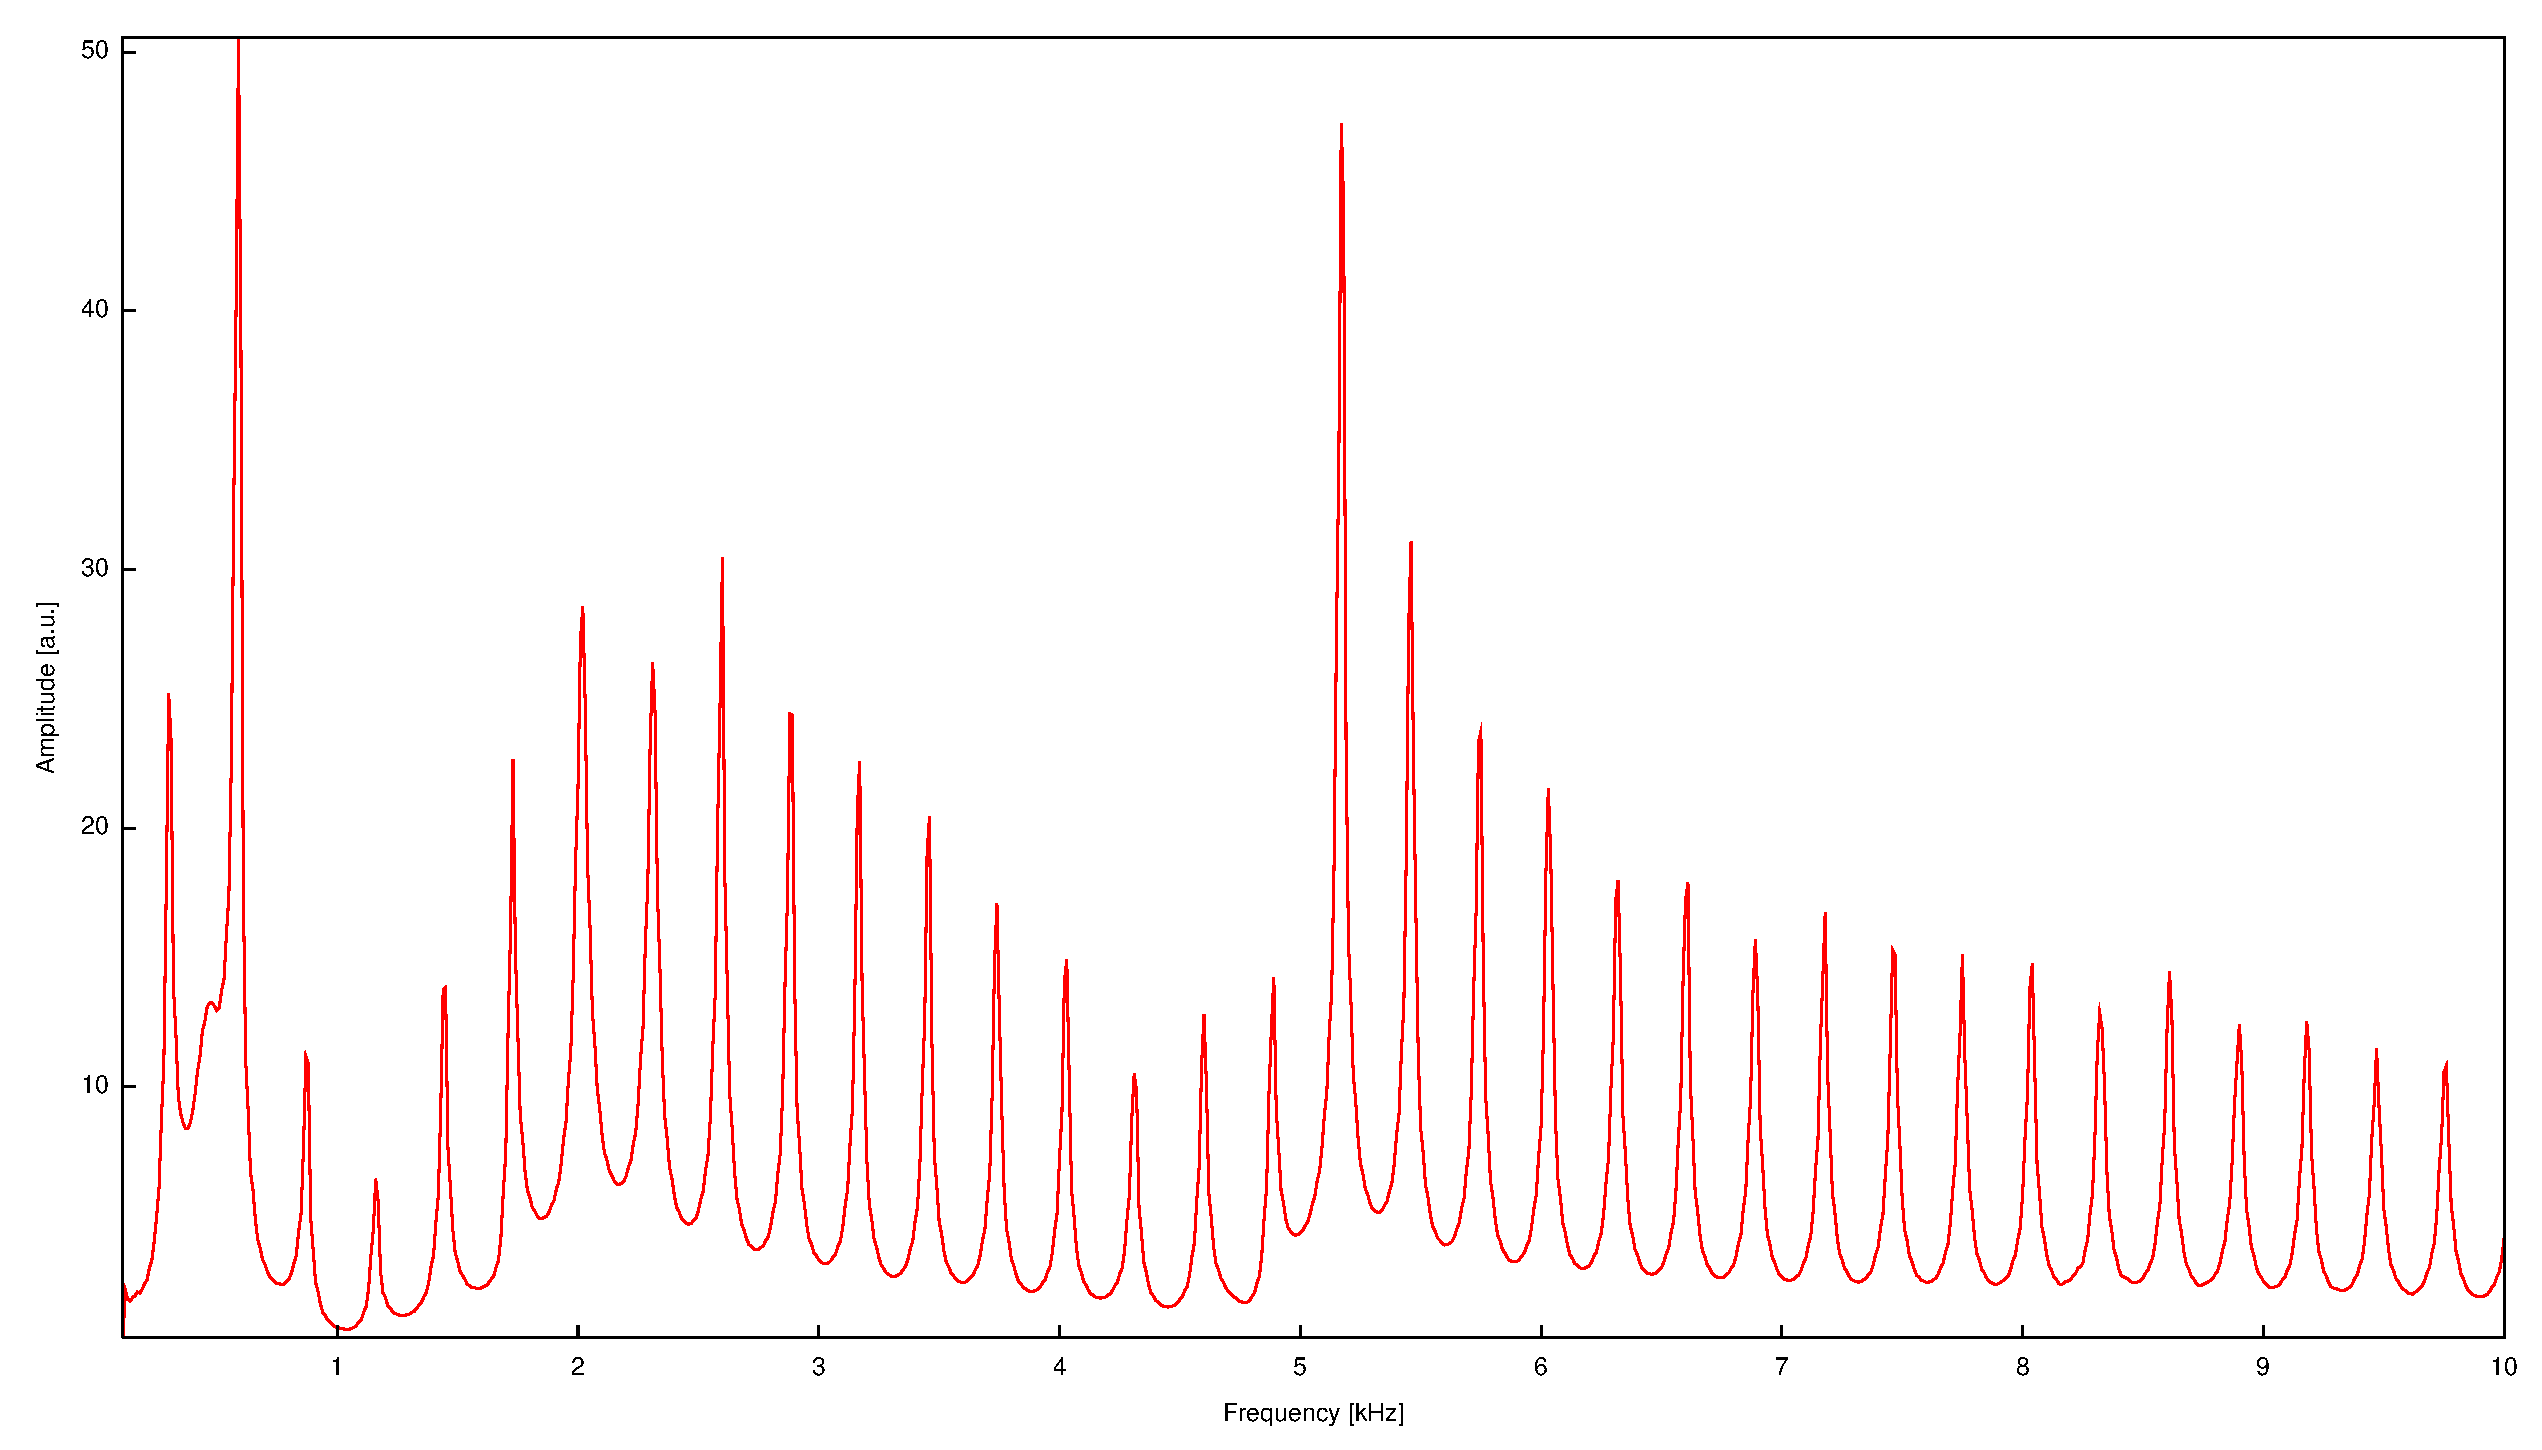
\includegraphics[scale=0.35]{FP-V23data/1.1_600mm.eps}
\caption{Spektrum einer $\SI{600}{\milli\meter}$-Röhre.}
\label{fig:Übersicht}
\end{figure}
\begin{figure}
\centering
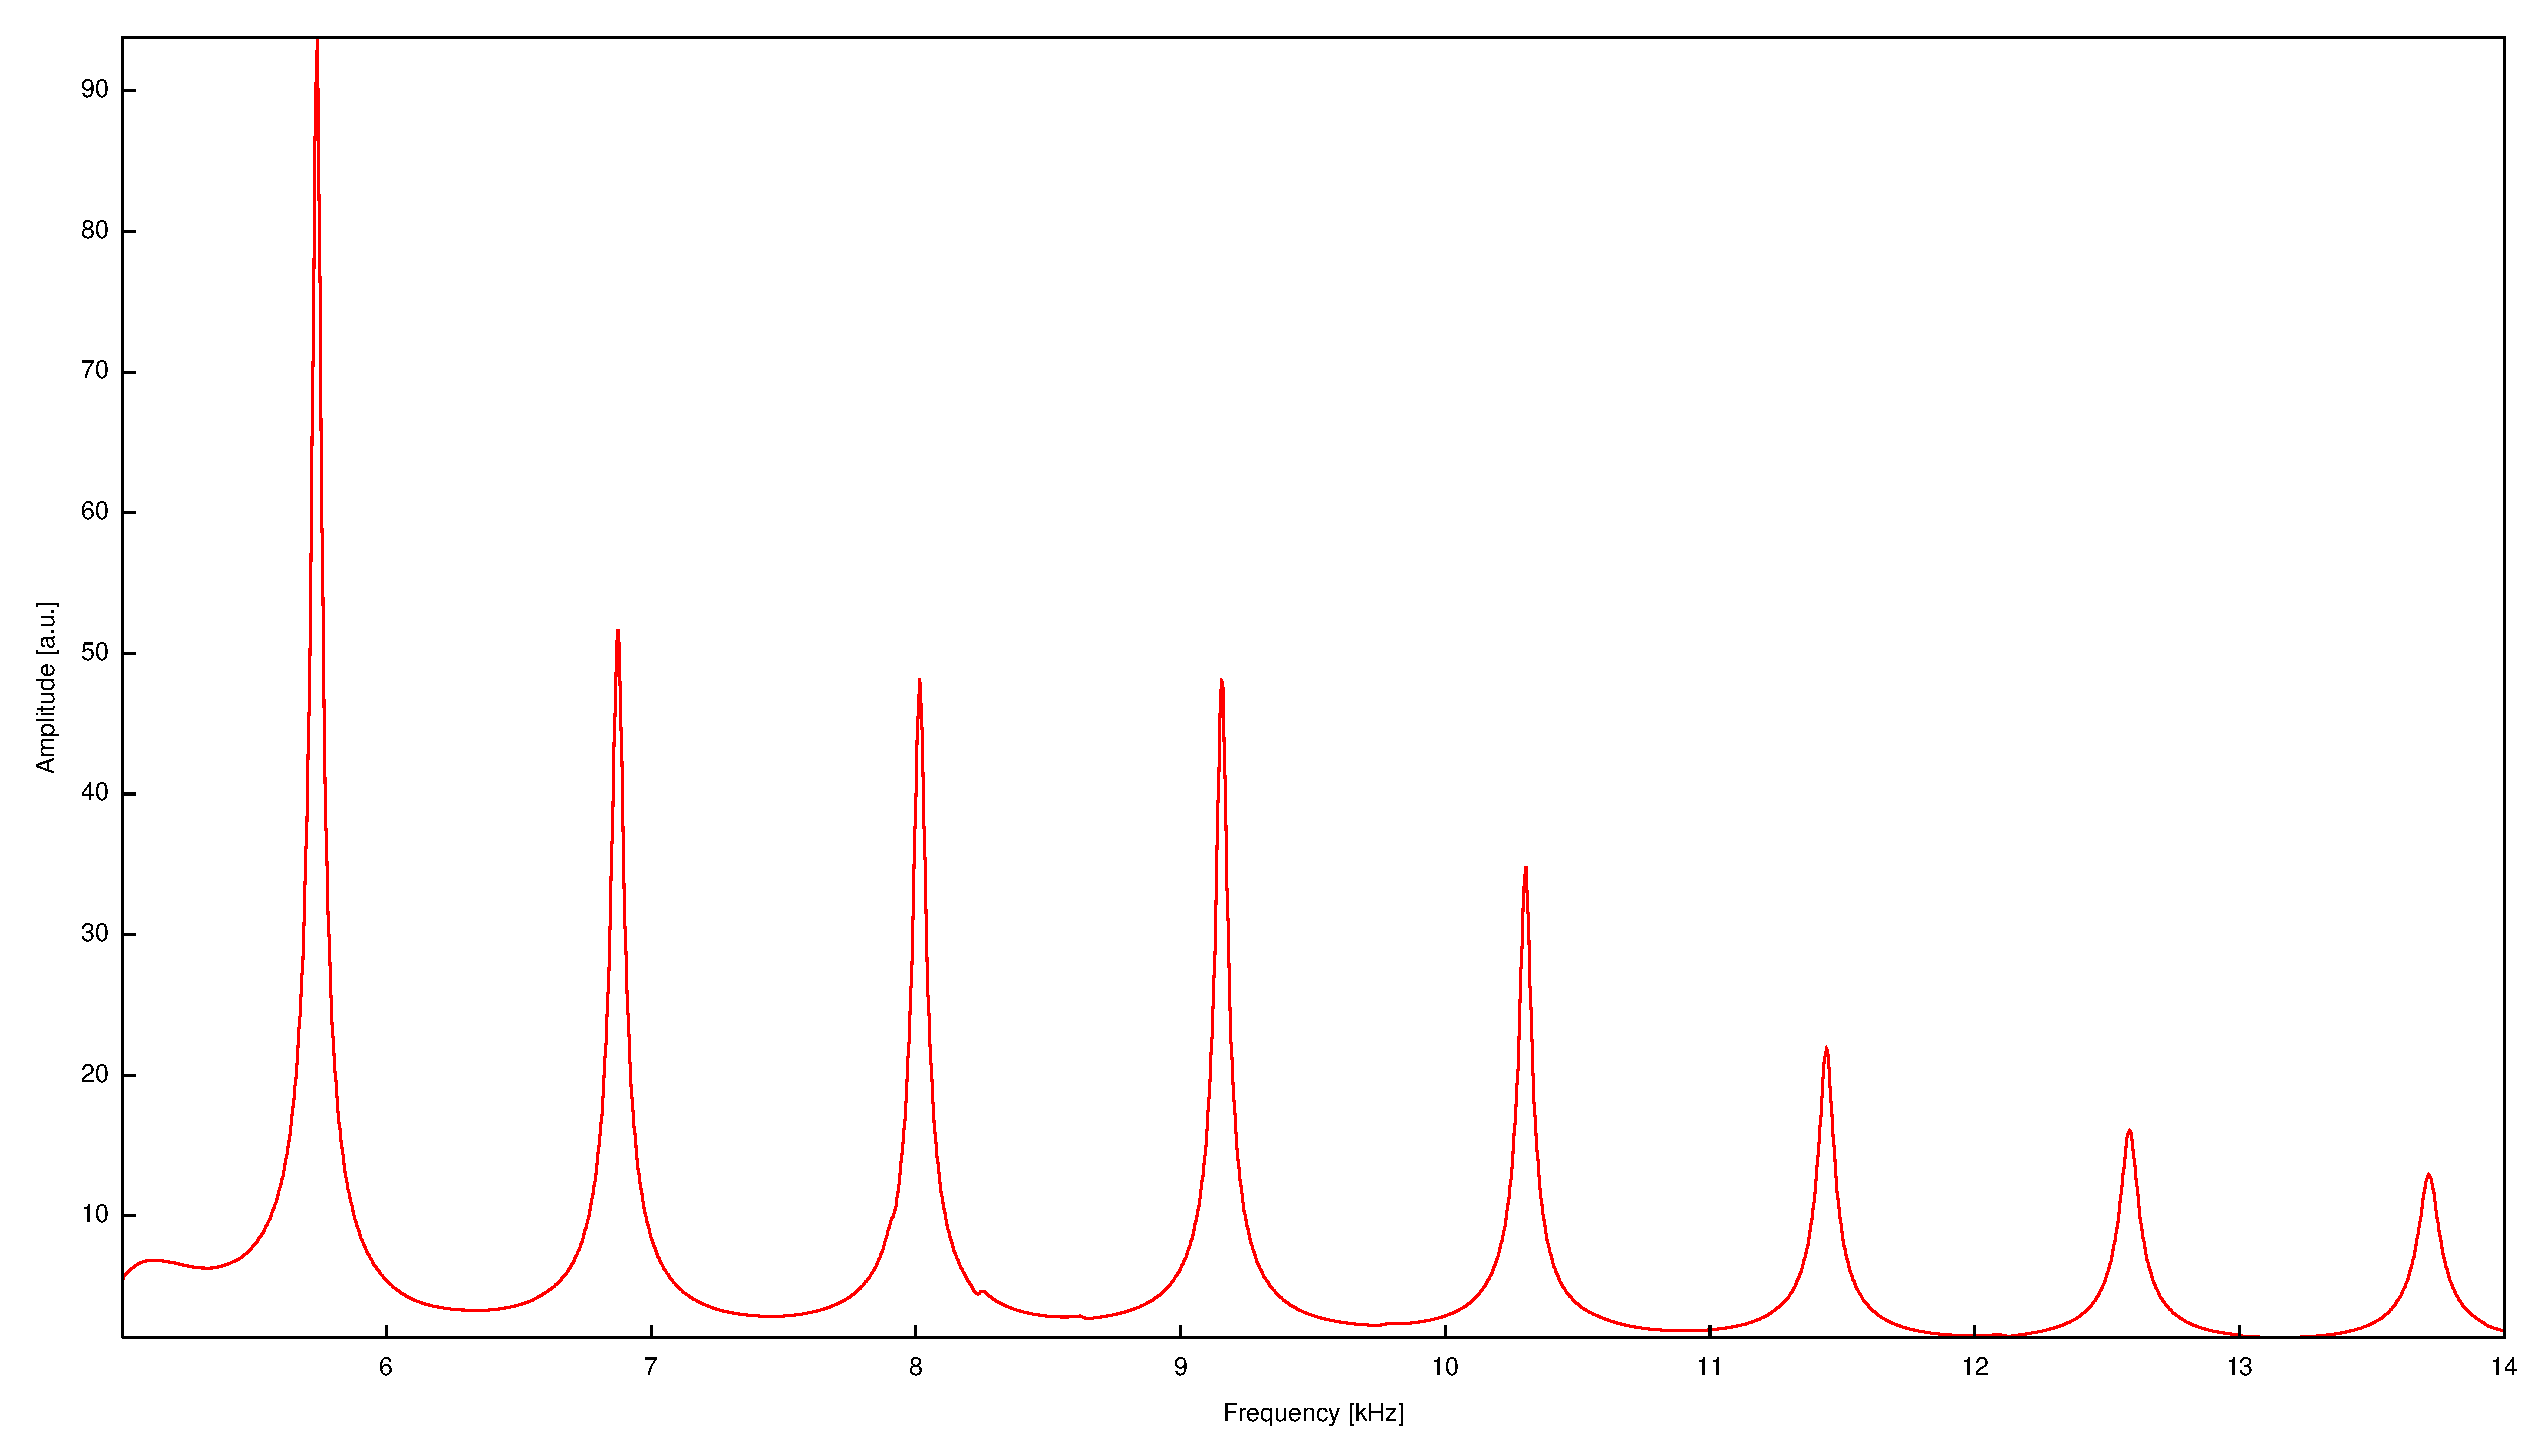
\includegraphics[scale=0.35]{FP-V23data/1.2(4.1)_150mm.eps}
\caption{Spektrum einer $\SI{150}{\milli\meter}$-Röhre.}
\label{fig:150}
\end{figure}
\begin{table}
\caption{Parameter des 1. Peaks von zwei spektralen Analysen einer $\SI{600}{\milli\meter}$ langen Röhre.}
\centering
\label{tab:params}
	\sisetup{table-format=1.2}
	\begin{tabular}{S[table-format=1.0]S[table-format=4.3]S[table-format=2.4]}
		\toprule
		{Messung} & {$f_\text{1}/(\si{\second^{-1}})$} & {$A_\text{1}/(\si{a.u.})$} \\
		\midrule
		 1 & 5747.706 & 92.8953 \\
		 2 & 5747.706 & 92.0576 \\
		\bottomrule
	\end{tabular}

\end{table}

\subsection{Modellierung: Das Wasserstoffatom}

In Abbildung \ref{fig:Overview} sind das Spektrum des sphärischen Resonators bei $\alpha=\SI{0}{\degree}$ und $\alpha=\SI{180}{\degree}$
zu sehen.
Die Resonanzfrequenzen $f_.n$ verändern sich nicht, jedoch fällt auf, dass bei $\alpha=\SI{0}{\degree}$ die Amplitude des 2. Peaks das Spektrum dominiert, während bei $\alpha=\SI{180}{\degree}$ alle Peaks in etwa dieselbe Höhe haben. Außerdem zeigt sich, dass in diesem Spektrum alle Peaks eine größere Amplitude aufweisen, als bei $\alpha=\SI{0}{\degree}$.\\
In Abbildung \ref{fig:5k_Peak1} und \ref{fig:5k_Peak2} ist für $\alpha=\SI{0}{\degree}$ und für $\alpha=\SI{40}{\degree}$, der Peak bei $f\approx\SI{5000}{\hertz}$ näher aufgelöst.
Es zeigt sich das der Hauptpeak mit zunehmendem $\alpha$ leicht zunimmt. Bei $\alpha=\SI{40}{\degree}$ bildet sich ein stark zunehmender Nebenpeak aus, der bei $\alpha=\SI{0}{\degree}$ von einer Einbuchtung überlagert wird.\\
In Abbildung \ref{fig:polar} sind die Polarplots der Peaks im Bereich von $\SI{2000}{\hertz}$ bis $\SI{7000}{\hertz}$ zu sehen.
Der Vergleich mit Bildern aus der Literatur\cite{V23}, liefert den Zusammenhang zwischen den ersten vier Peaks und den Kugelflächenfunktionen:
\begin{align*}
.{Peak 1}&\mathop{\widehat{=}} Y^0_1\\
.{Peak 2}&\mathop{\widehat{=}} Y^0_2\\
.{Peak 3}&\mathop{\widehat{=}} Y^0_3\\
.{Peak 4}&\mathop{\widehat{=}} Y^0_4\\
\end{align*}
Der 5. Polarplot lässt sich keinem Zustand mit $m=0$ zuordnen und ähnelt am ehesten der Kugelflächenfunktion $Y^.1_.2$.
\begin{figure}
\centering
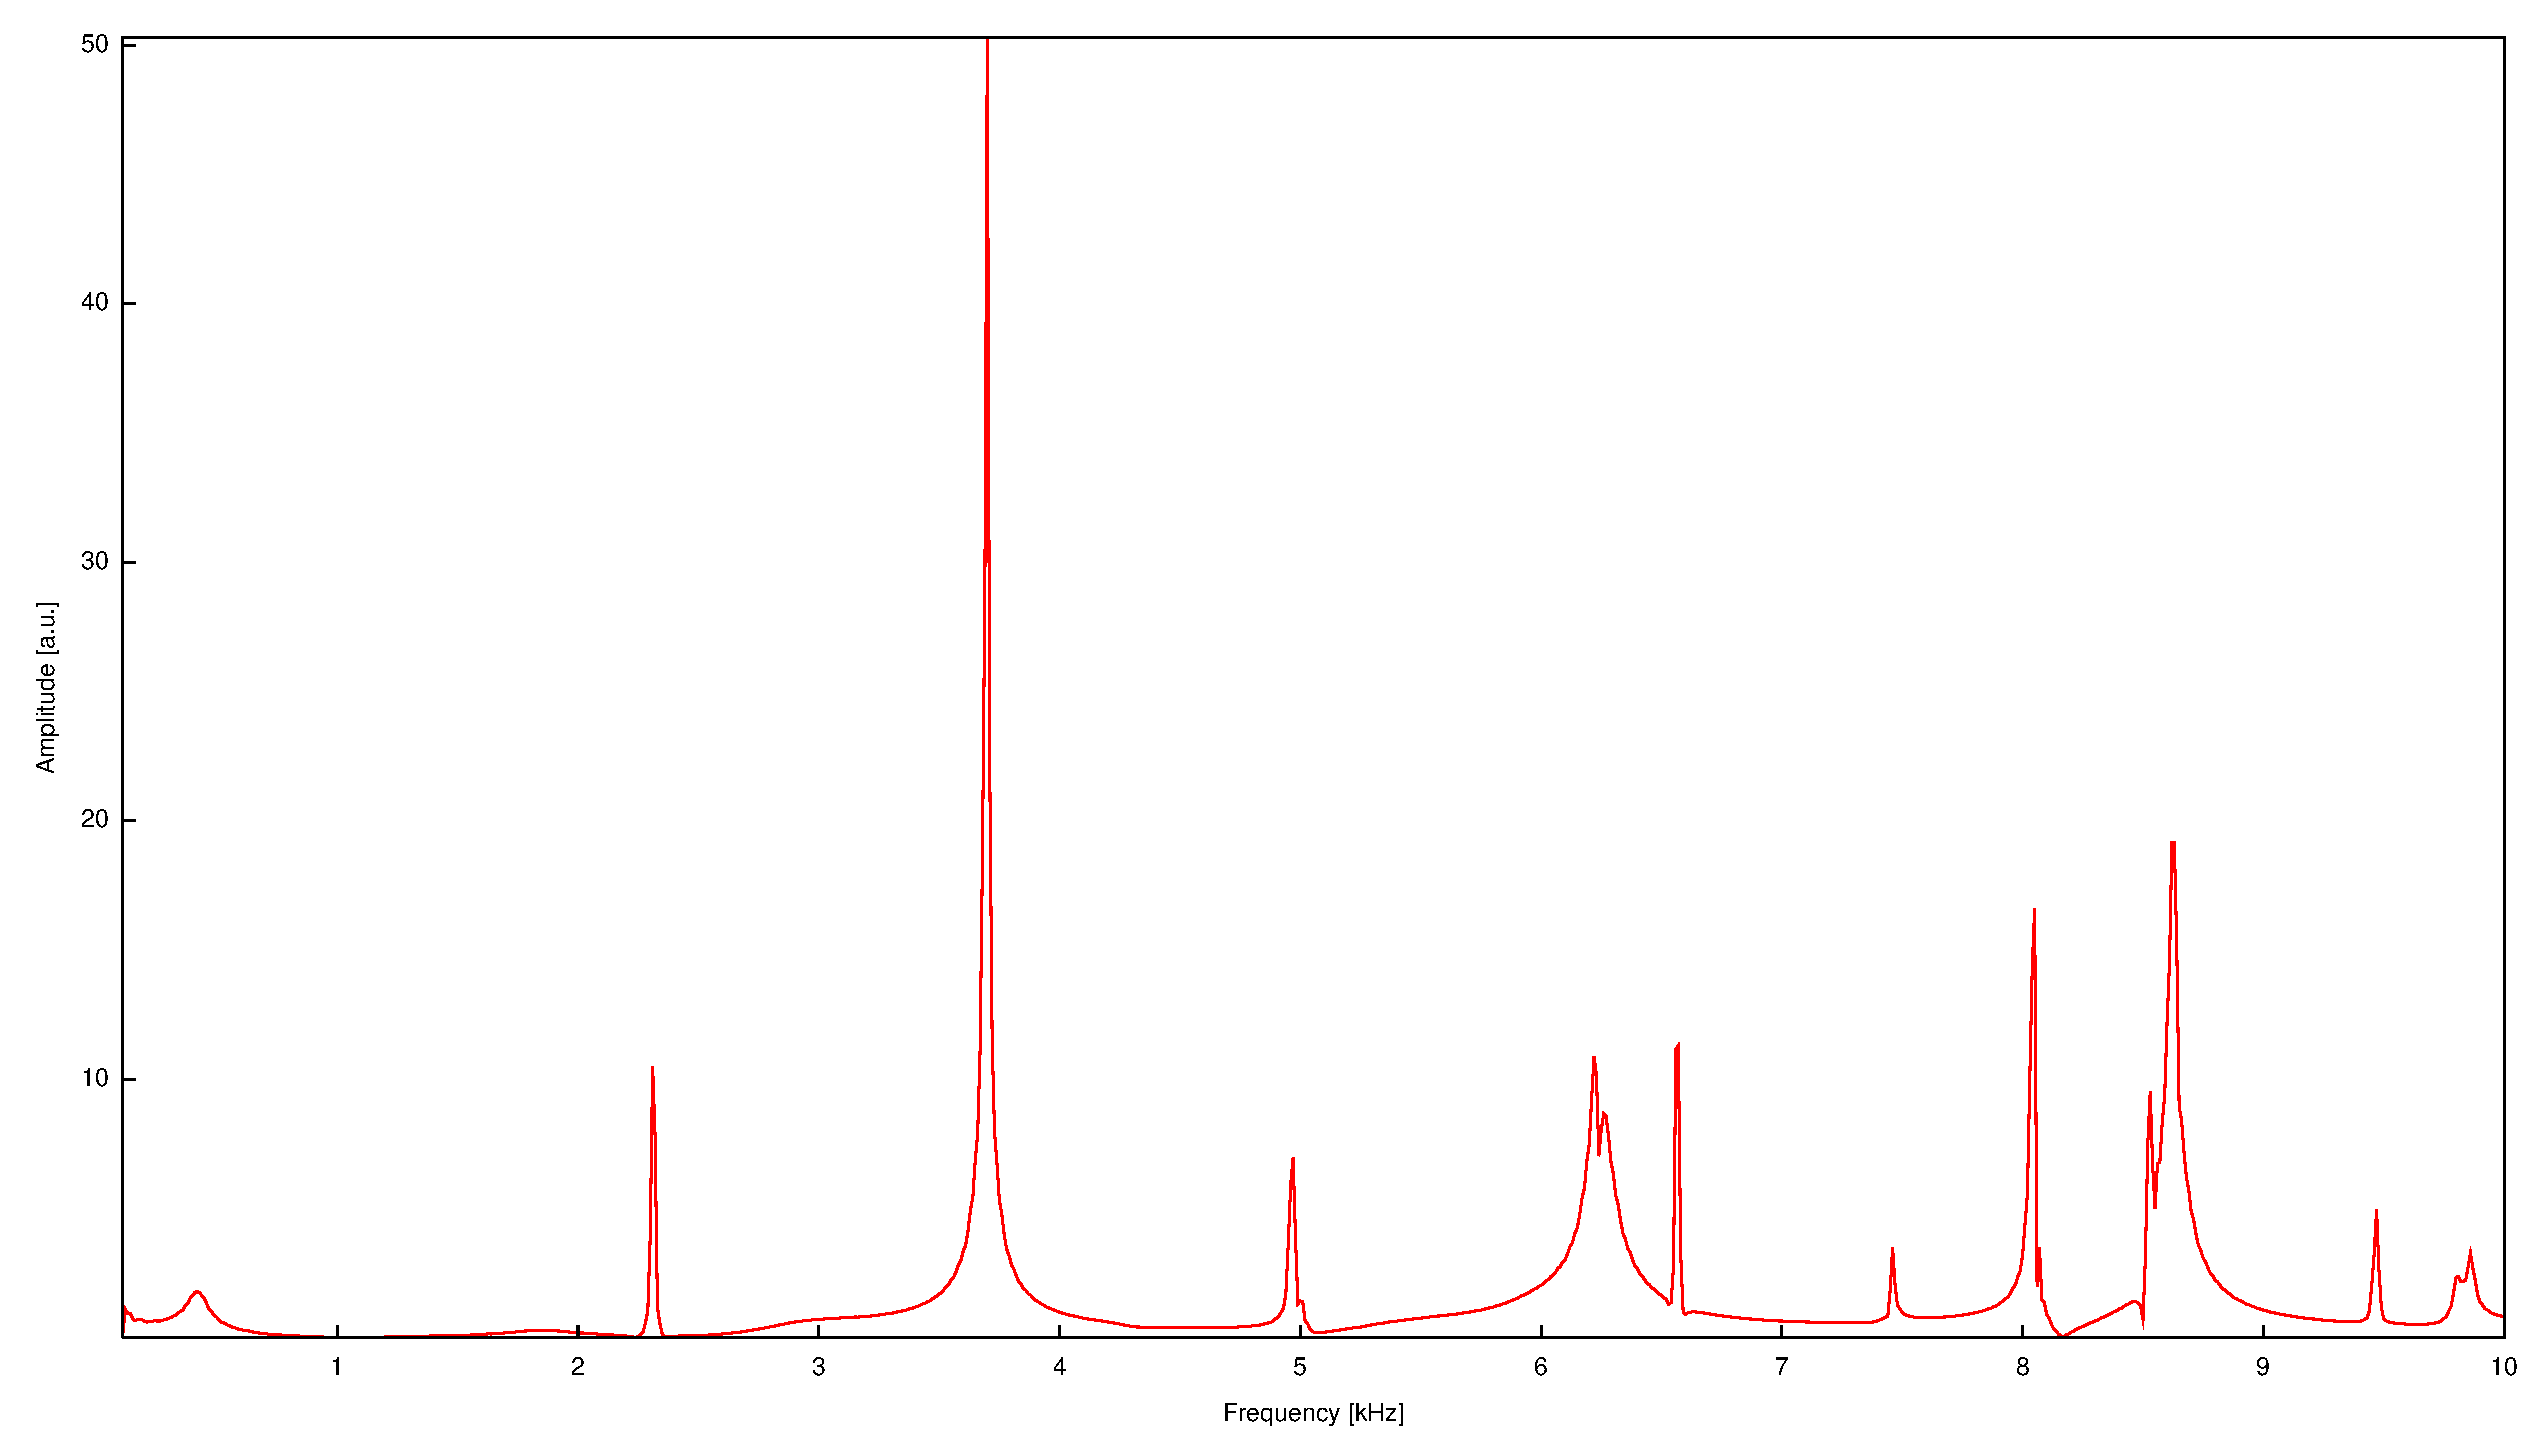
\includegraphics[scale=0.35]{FP-V23data/2.1_0degree.eps}
\caption{Spektrum im sphärischen Resonate für $\alpha=\SI{0}{\degree}$.}
\label{fig:Overview1}
\end{figure}
\begin{figure}
\centering
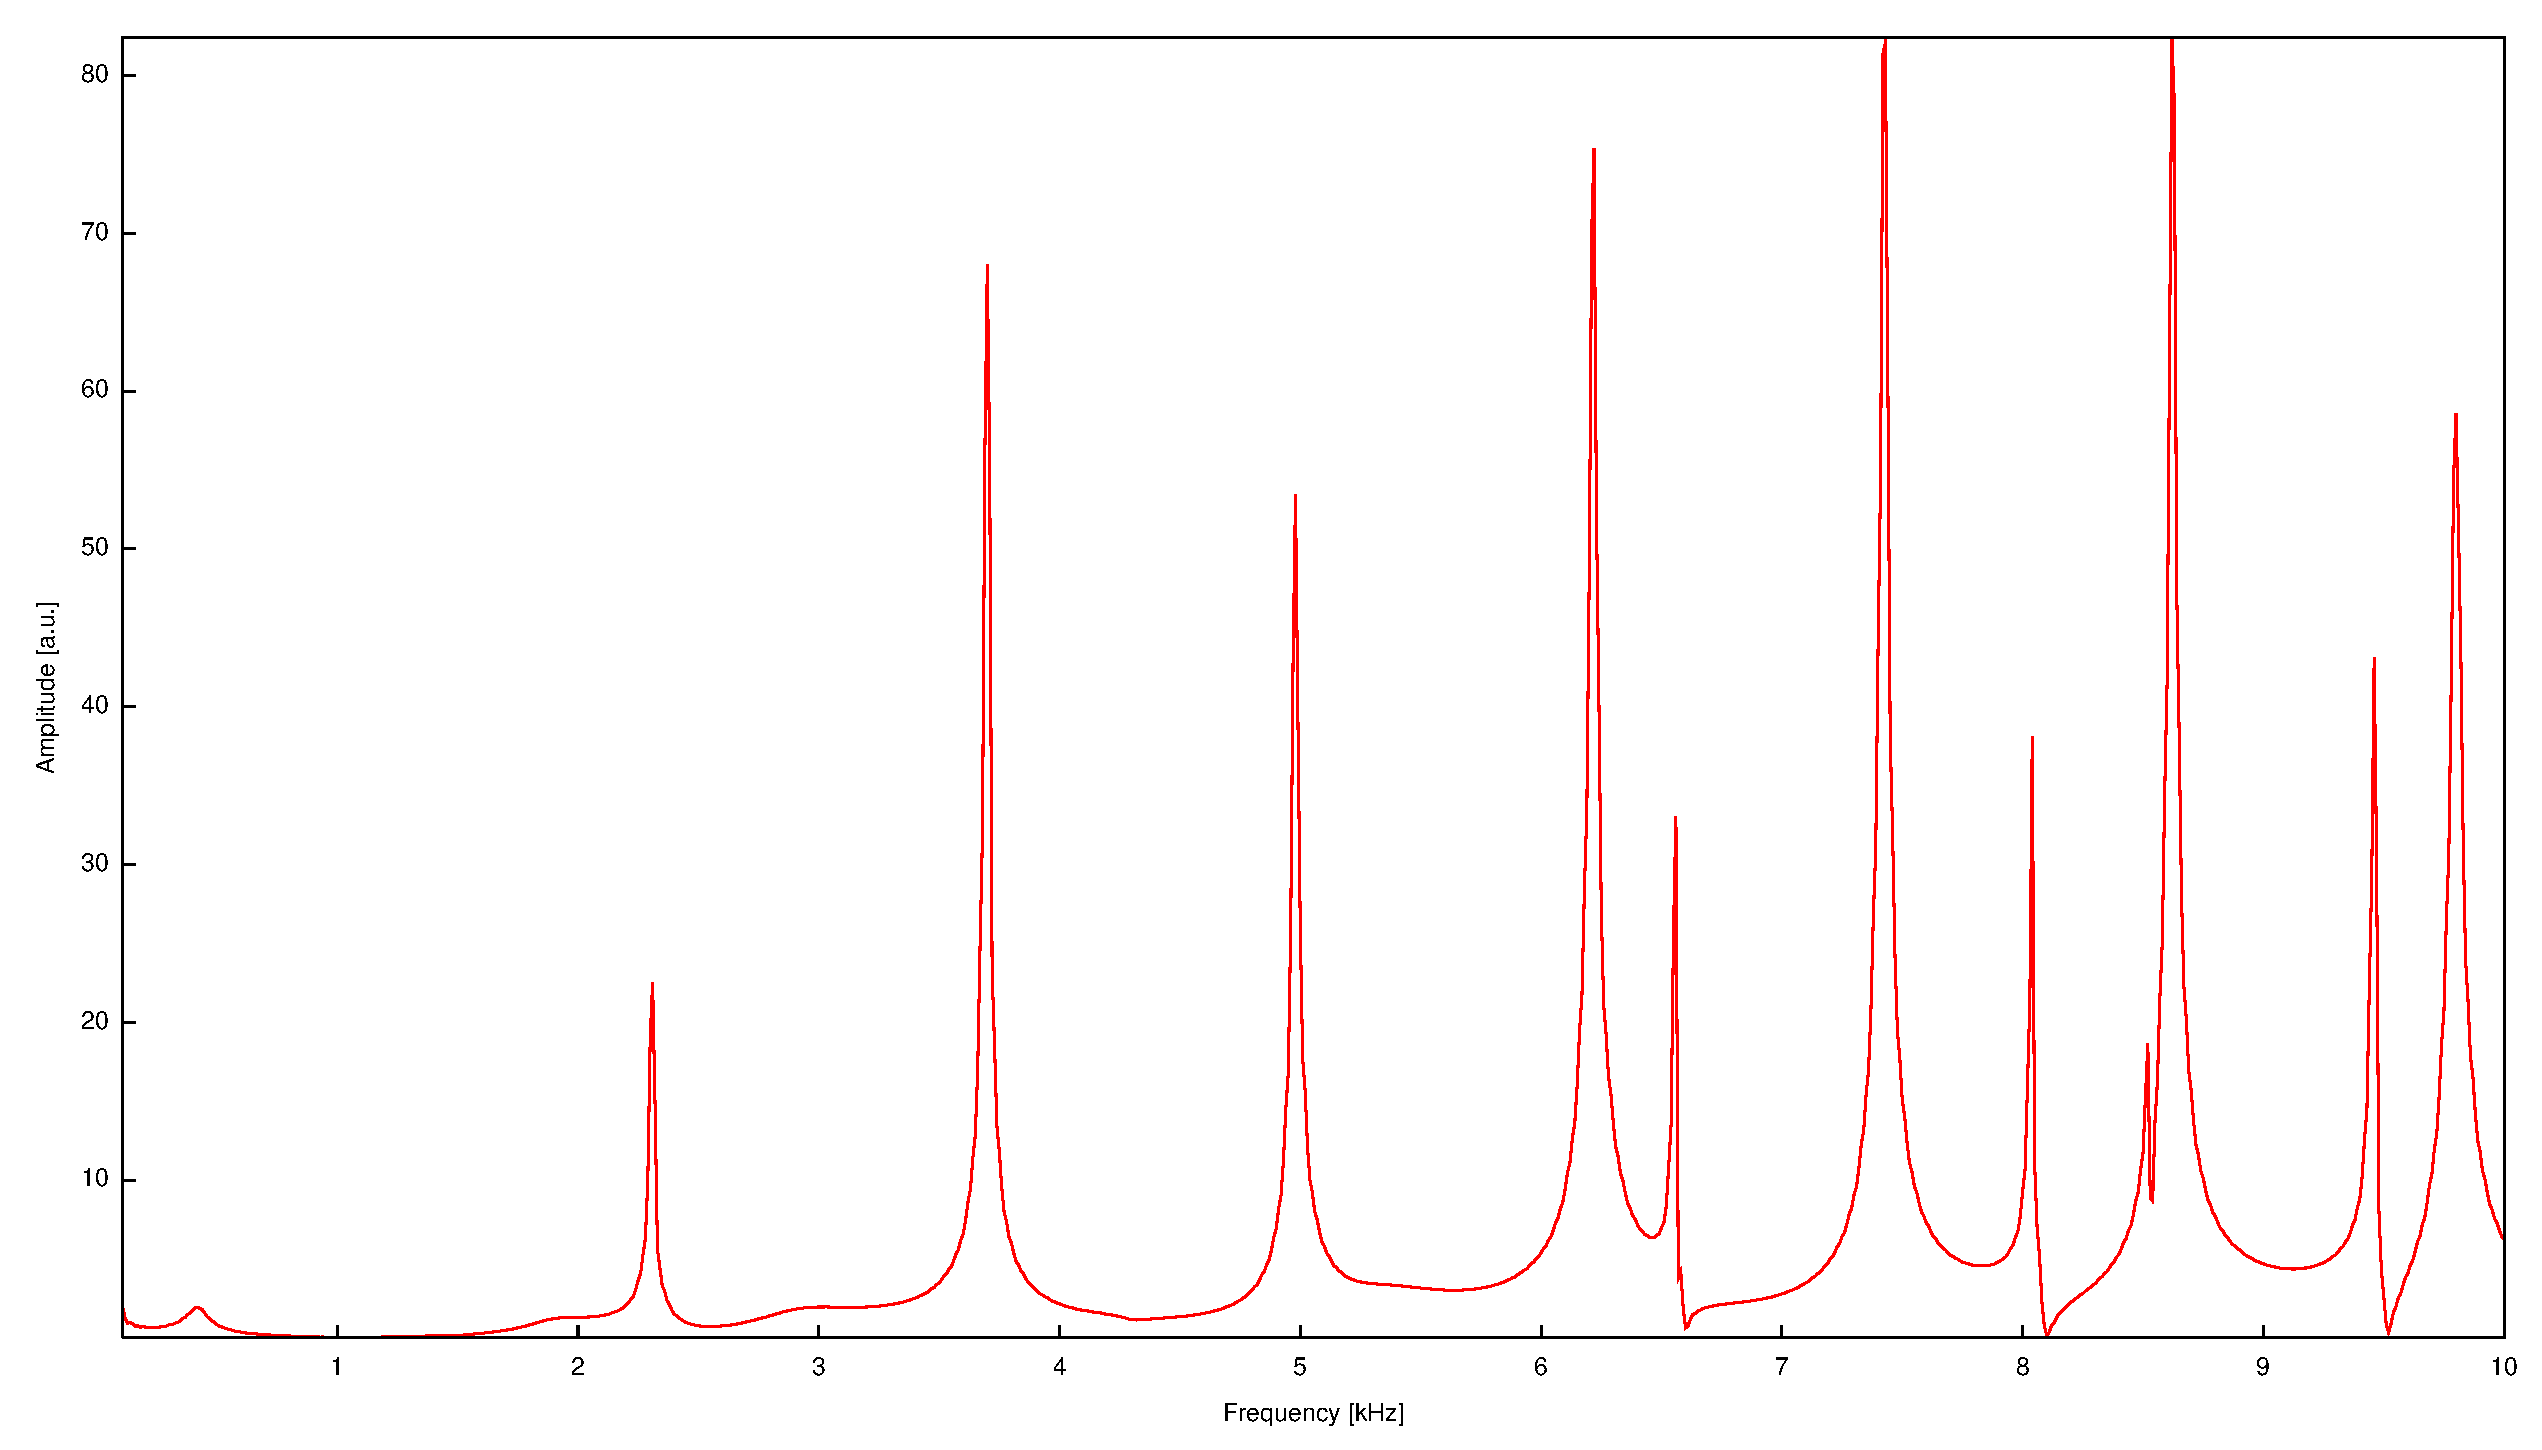
\includegraphics[scale=0.35]{FP-V23data/2.1_180degree.eps}
\caption{Spektrum im sphärischen Resonate für $\alpha=\SI{180}{\degree}$.}
\label{fig:Overview2}
\end{figure}
\begin{figure}
\centering
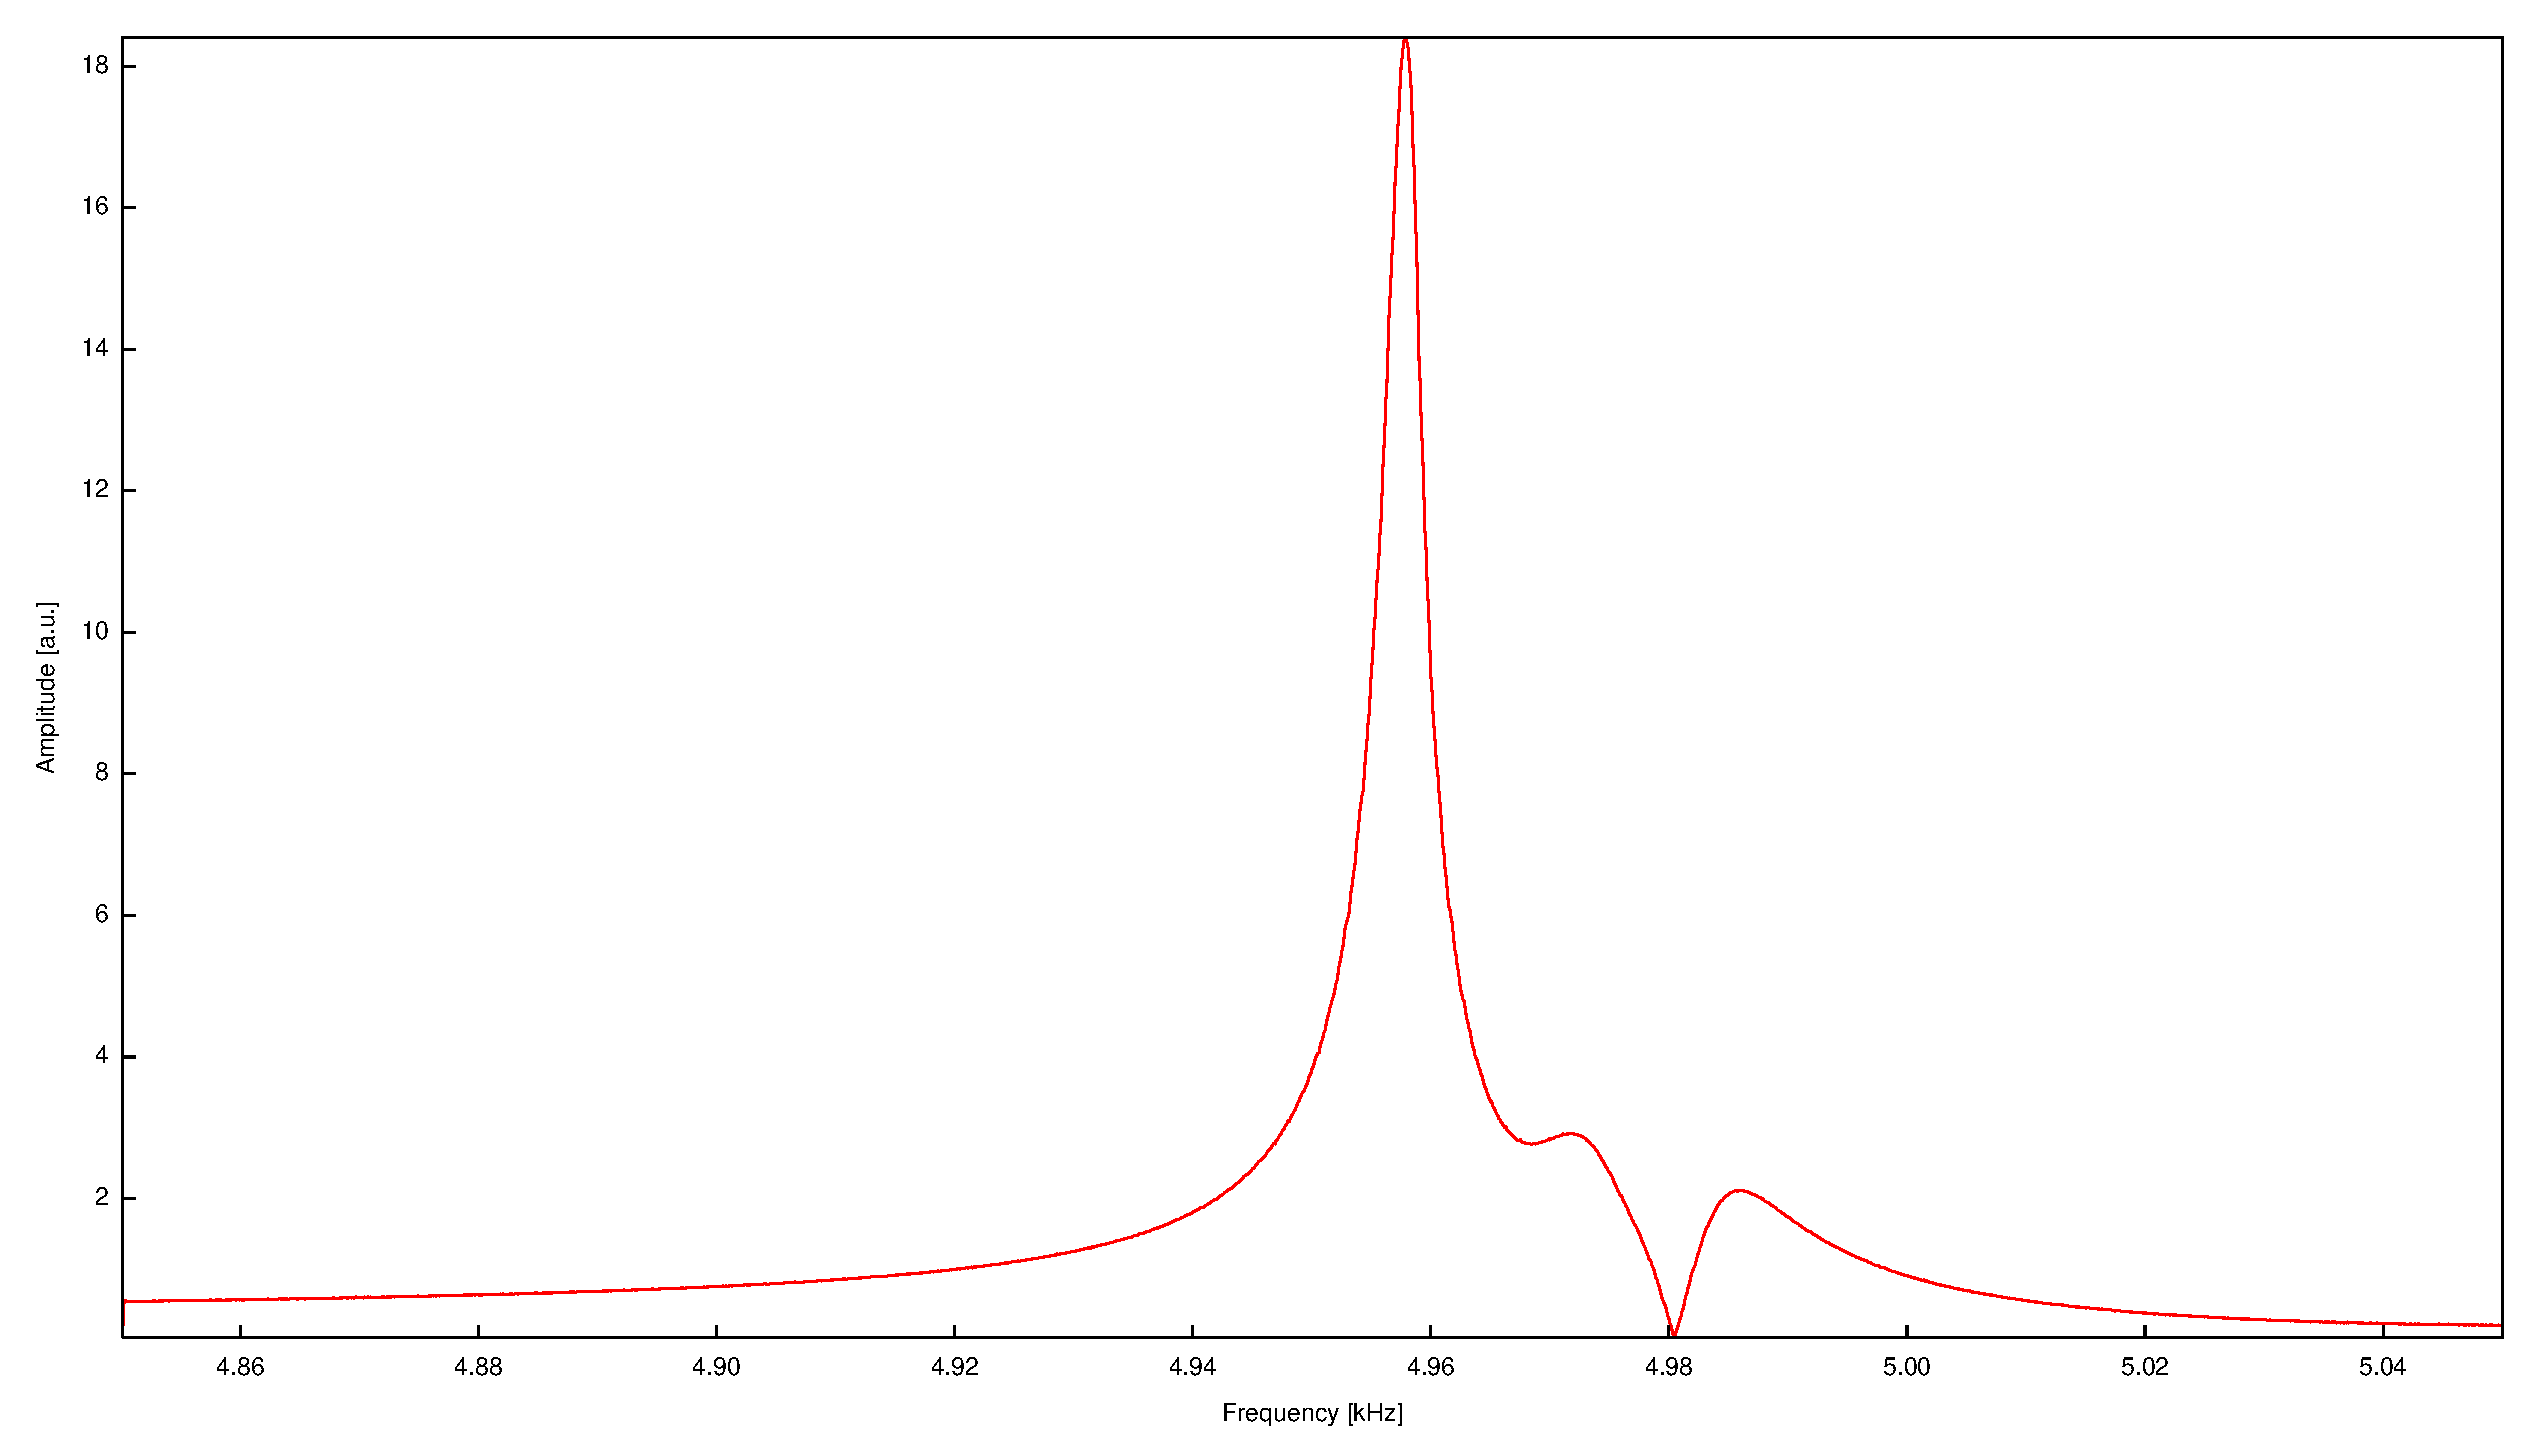
\includegraphics[scale=0.35]{FP-V23data/2.2_0degree.eps}
\caption{Nähere Aufnahme des Peaks bei $f\approx\SI{5000}{\hertz}$ für $\alpha=\SI{0}{\degree}$.}
\label{fig:5k_Peak1}
\end{figure}
\begin{figure}
\centering
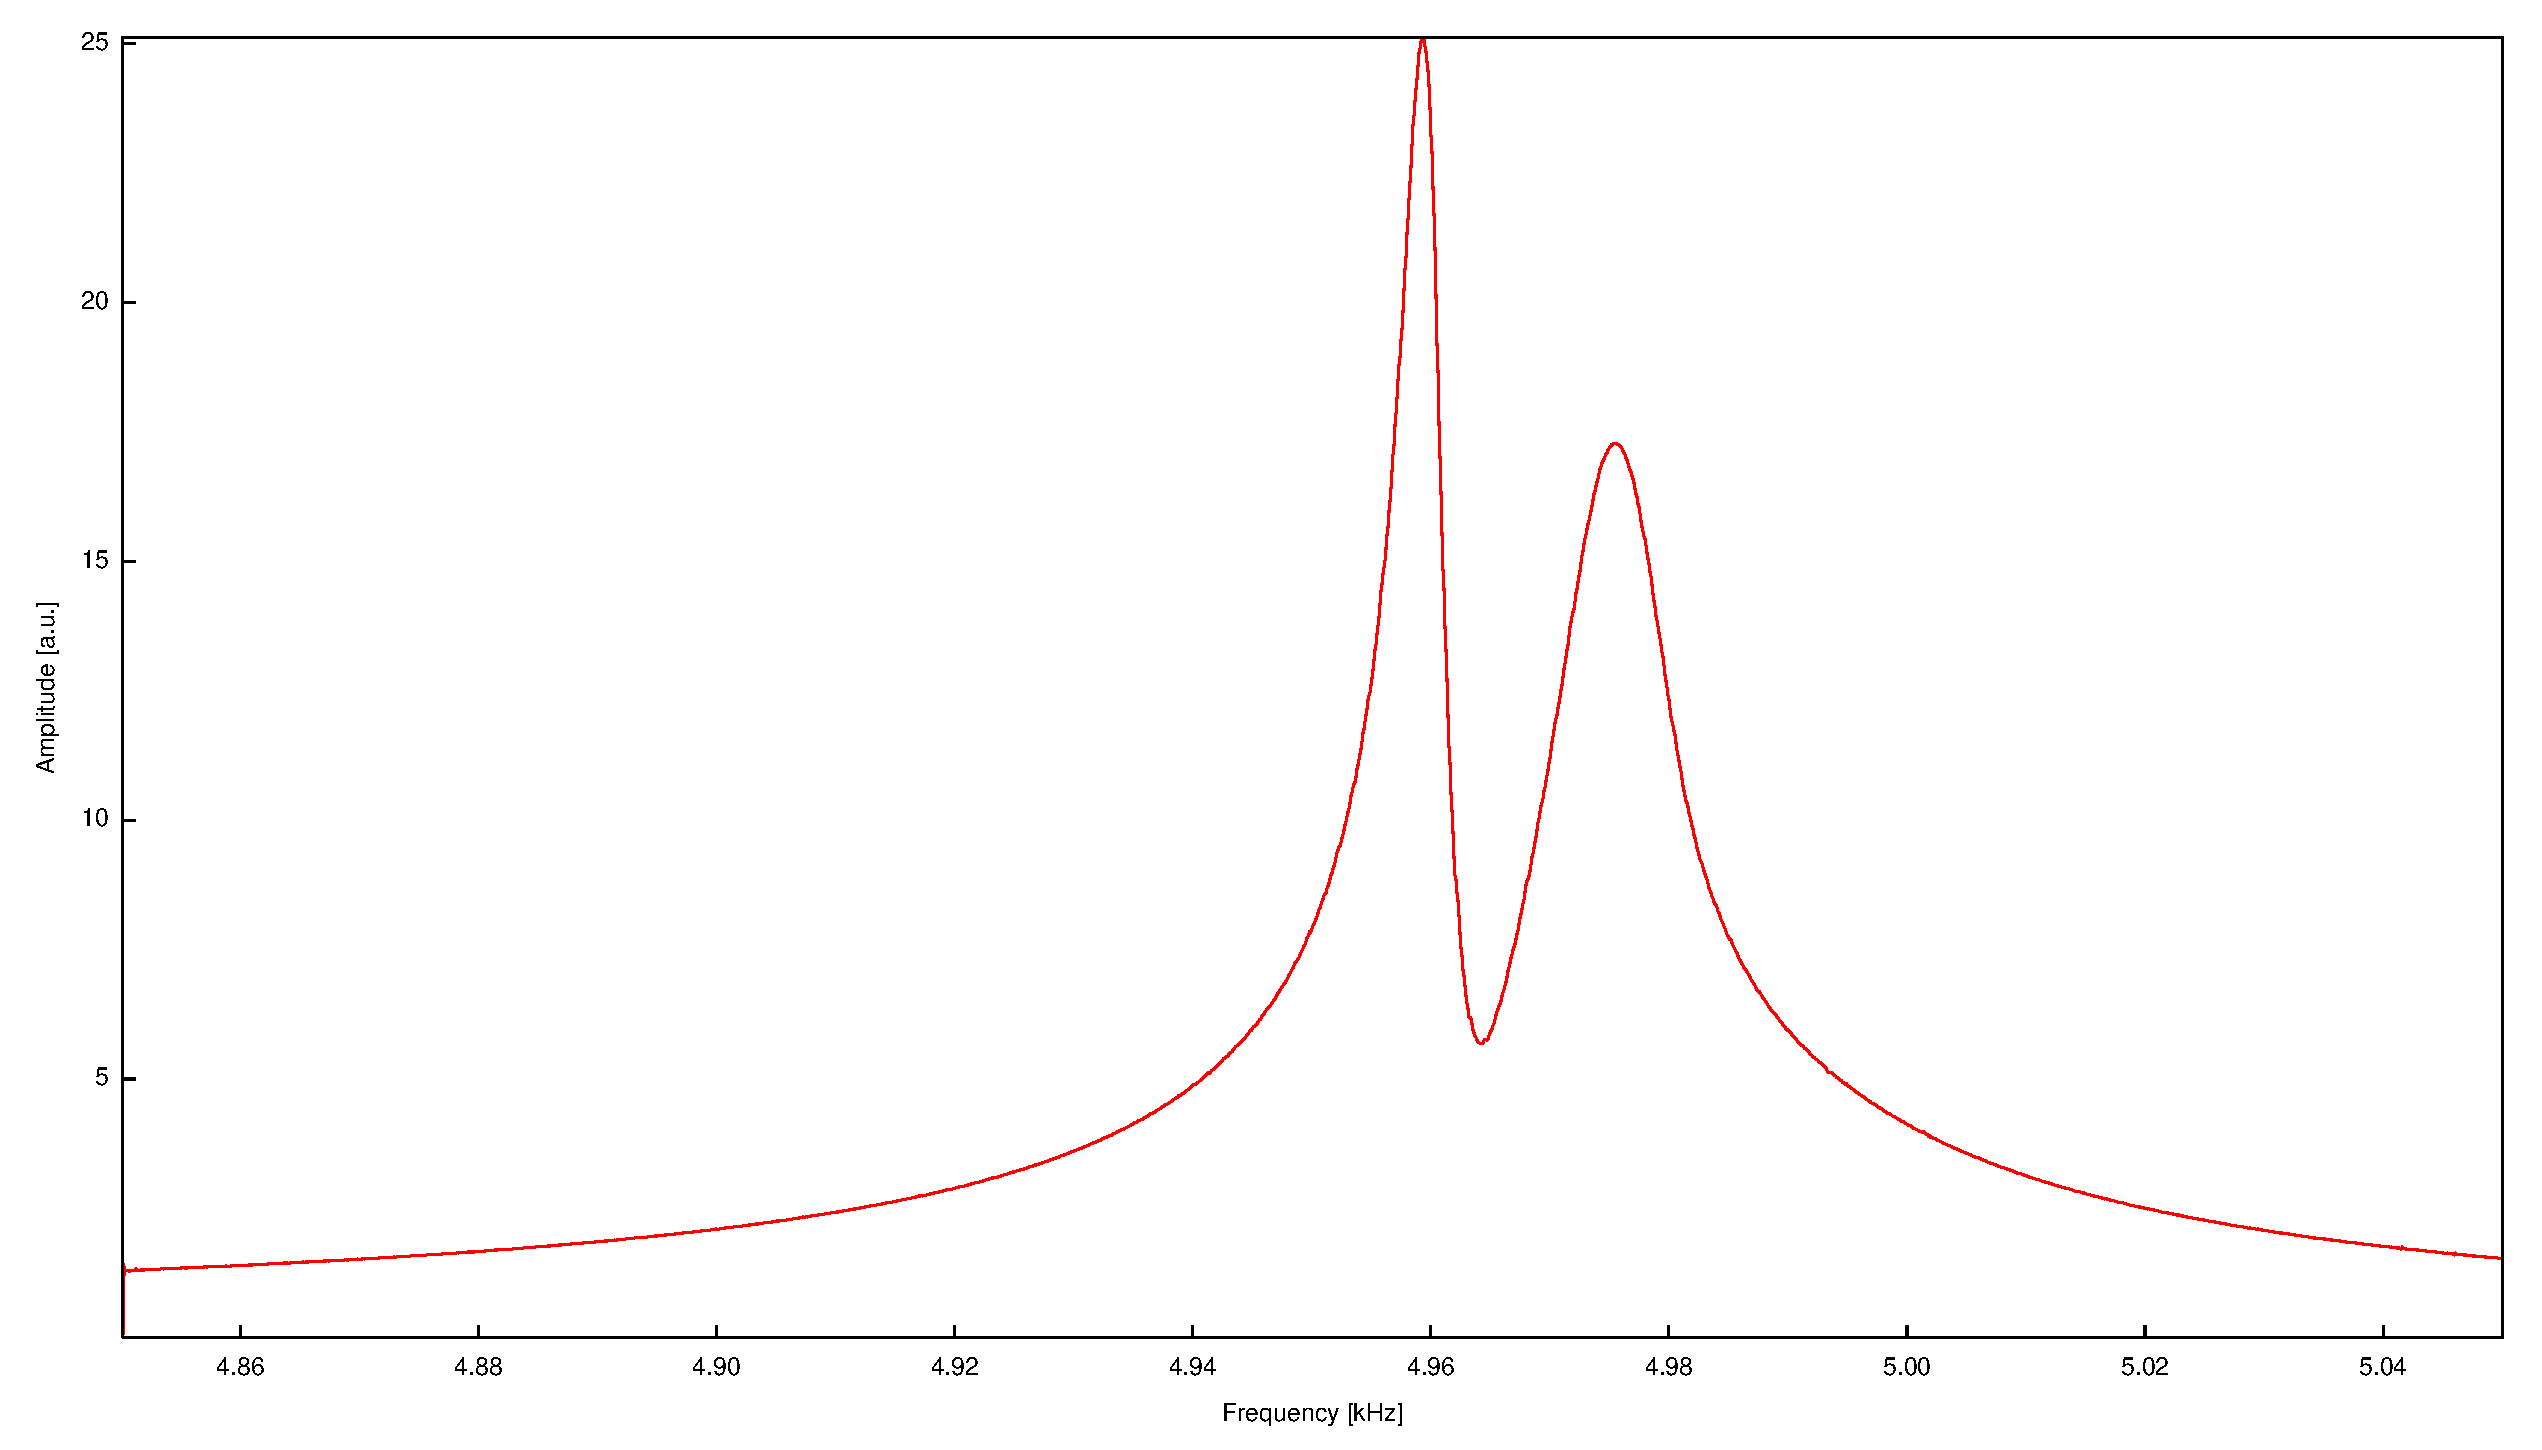
\includegraphics[scale=0.35]{FP-V23data/2.2_40degree.eps}
\caption{Nähere Aufnahme des Peaks bei $f\approx\SI{5000}{\hertz}$ für $\alpha=\SI{40}{\degree}$.}
\label{fig:5k_Peak2}
\end{figure}
\begin{figure}
\centering
\begin{minipage}{0.45\textwidth}
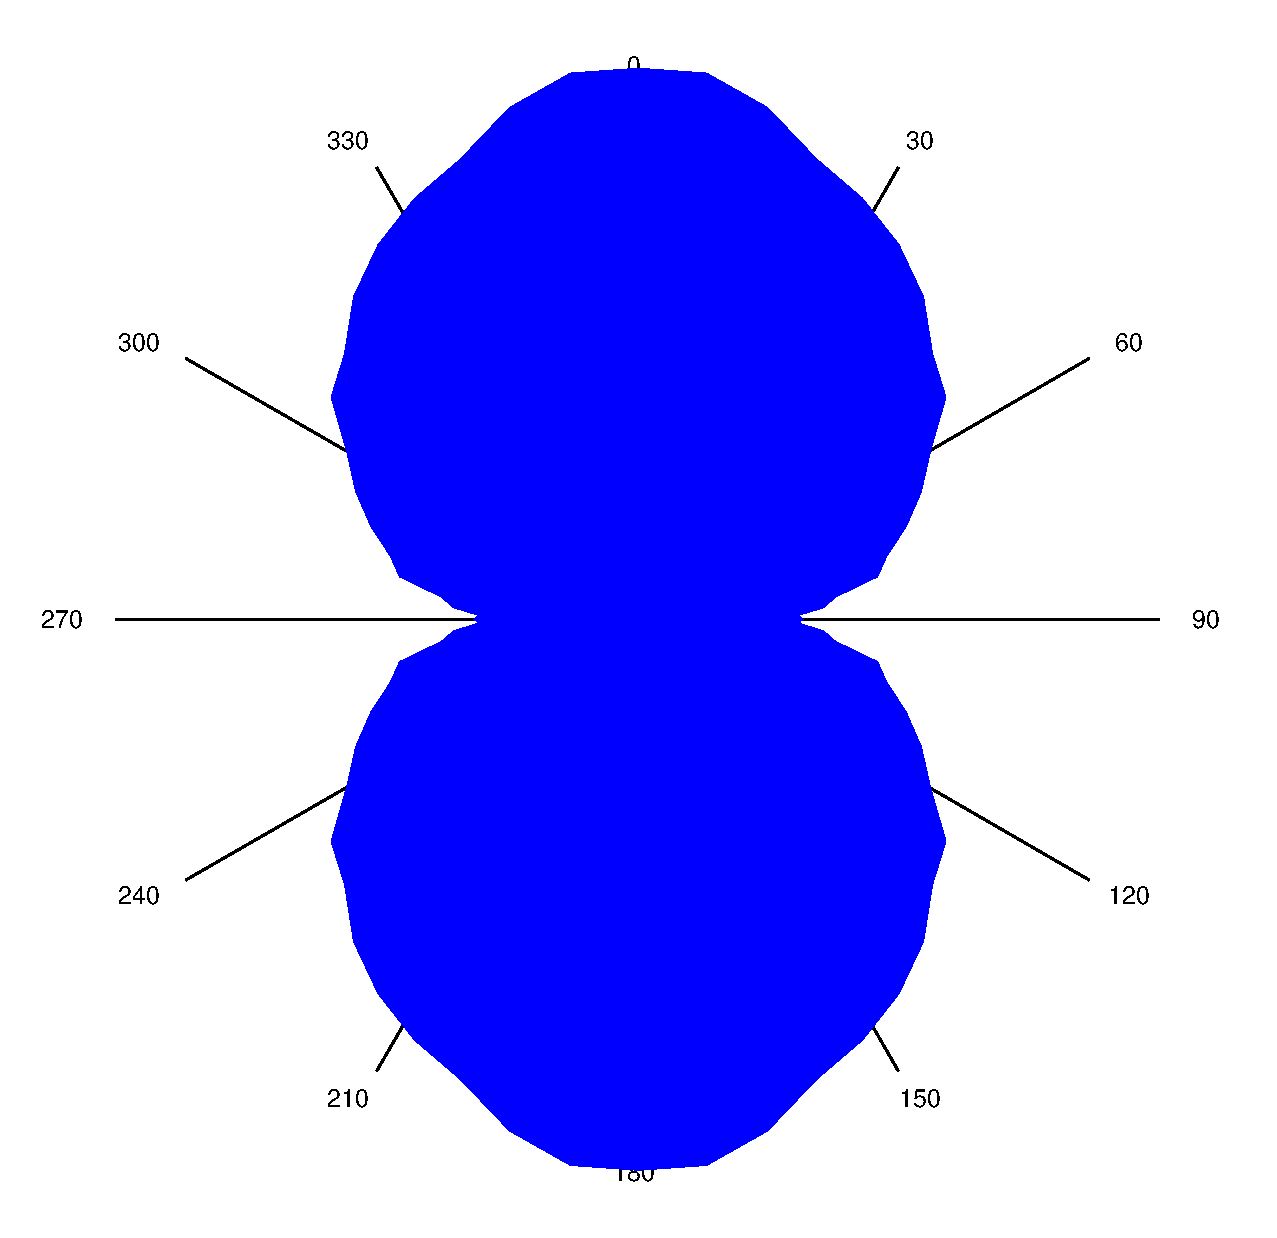
\includegraphics[scale=0.2]{FP-V23data/2.3_2306.535Hz.eps}
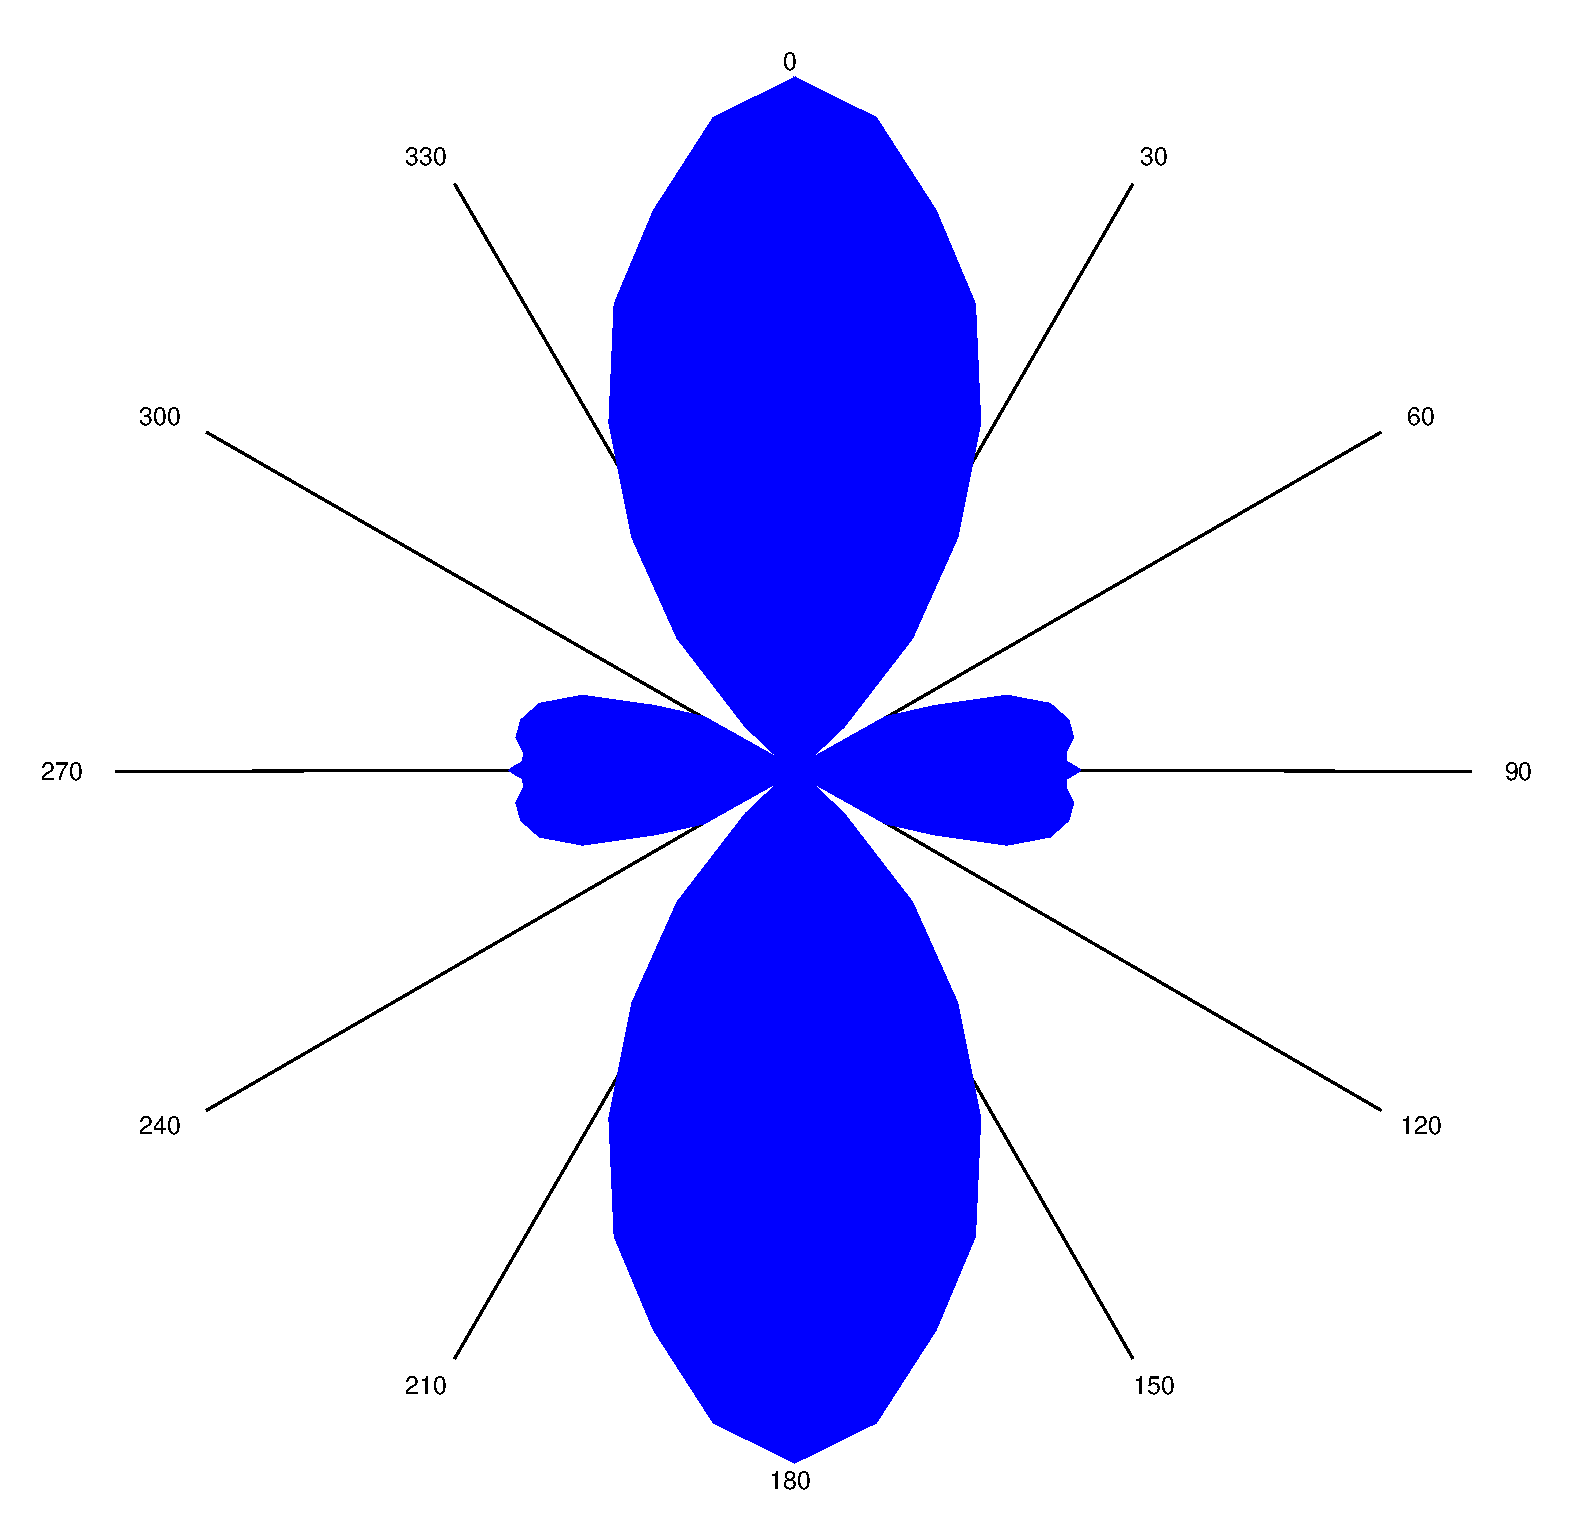
\includegraphics[scale=0.2]{FP-V23data/2.3_3704.961Hz.eps}
\end{minipage}
\begin{minipage}{0.45\textwidth}
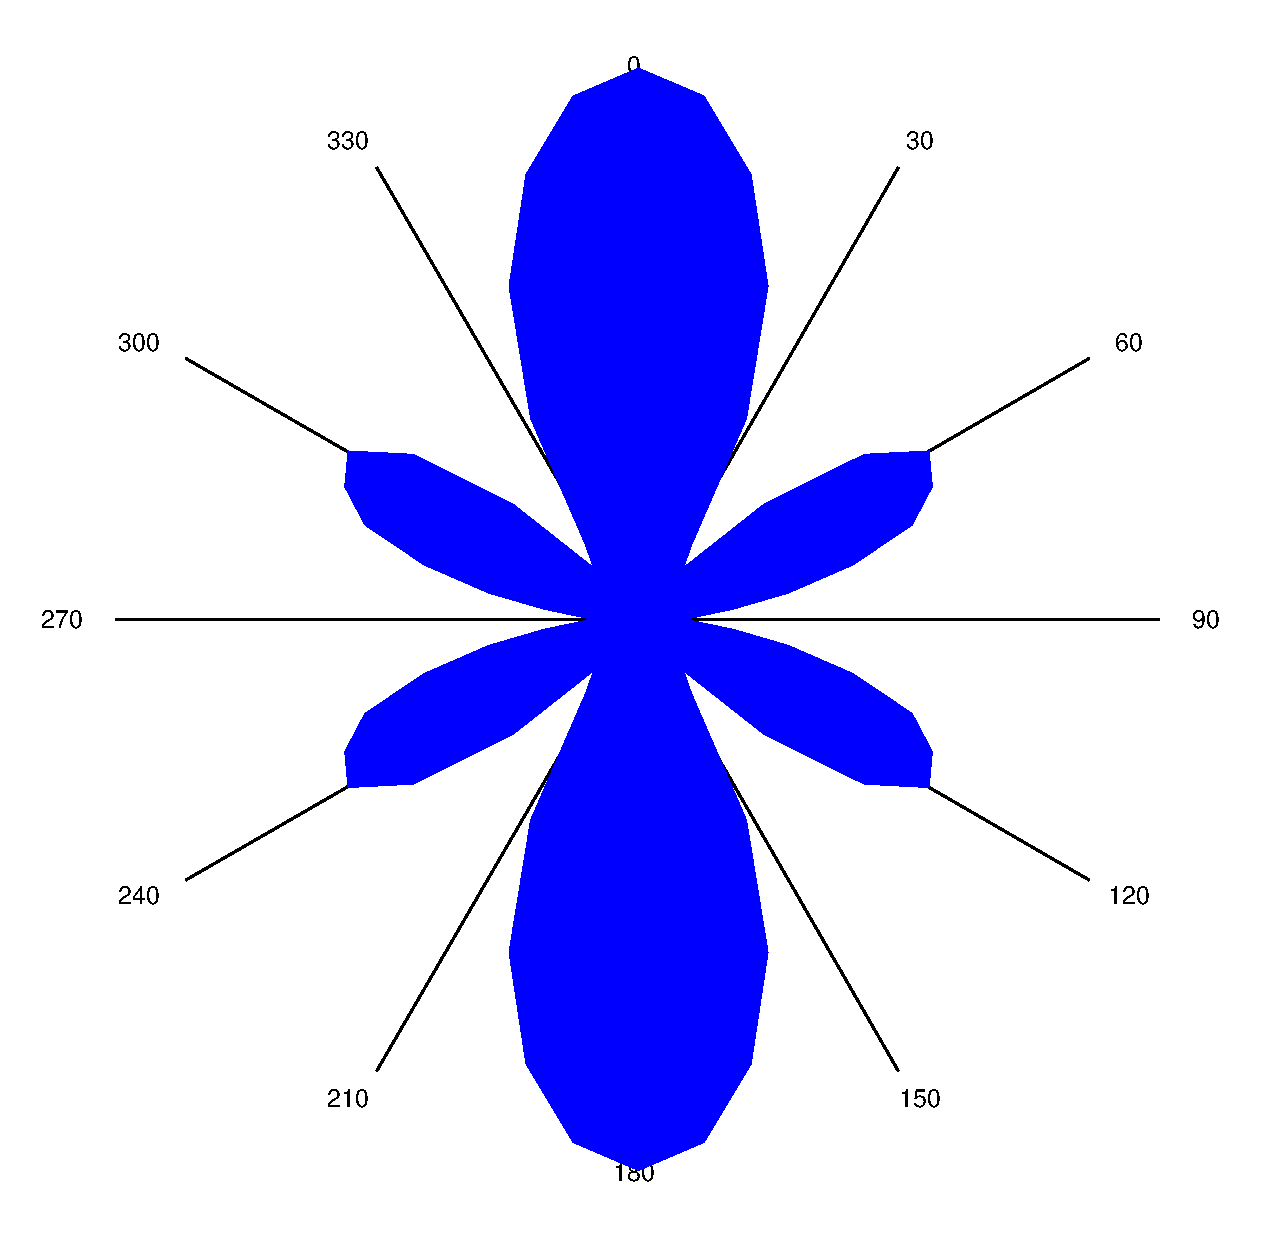
\includegraphics[scale=0.2]{FP-V23data/2.3_4985.394Hz.eps}
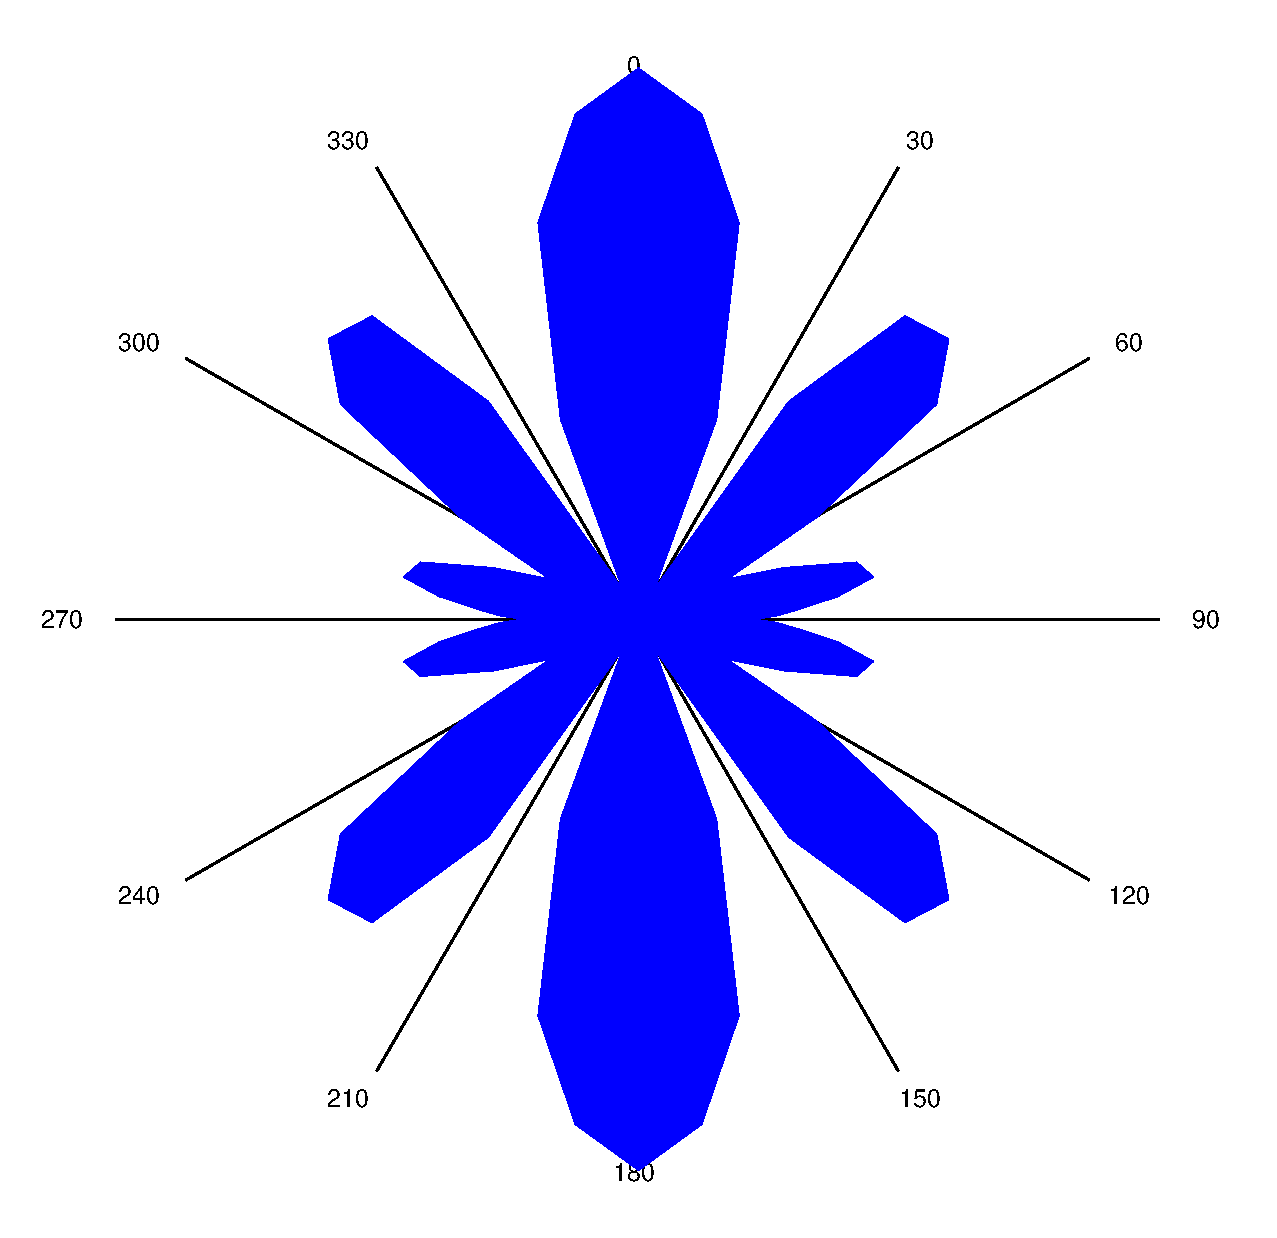
\includegraphics[scale=0.2]{FP-V23data/2.3_6230.866Hz.eps}
\end{minipage}
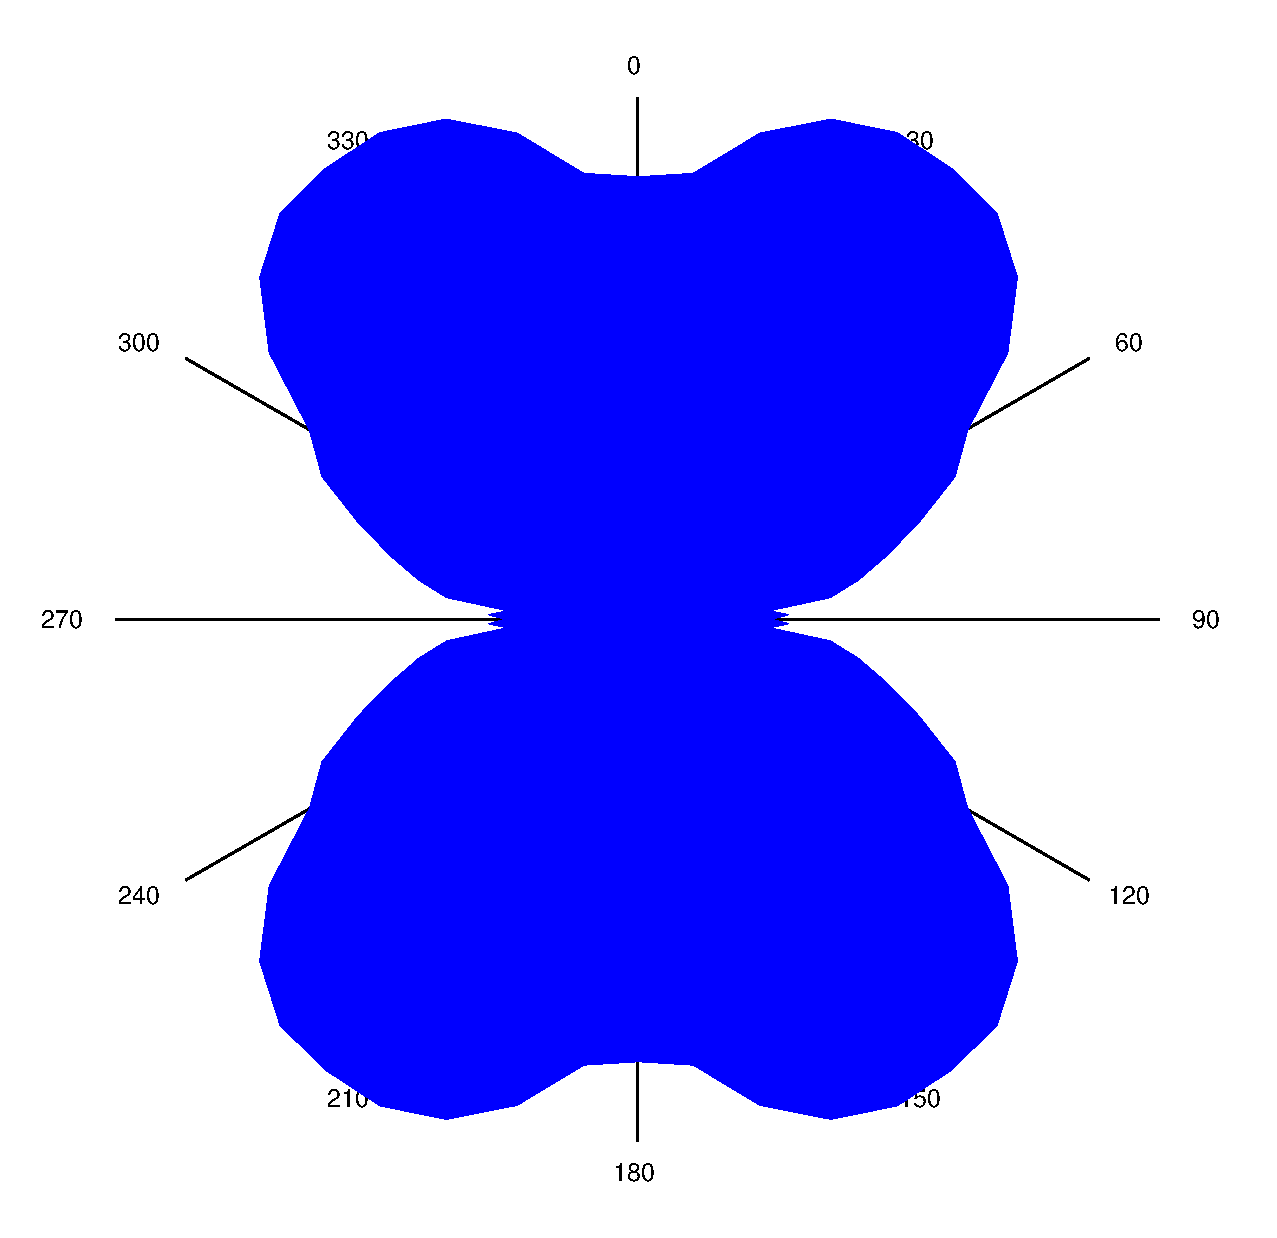
\includegraphics[scale=0.2]{FP-V23data/2.3_6571.732Hz.eps}
\caption{Polarplots der ersten fünf Peaks im sphärischen Resonator}
\label{fig:polar}
\end{figure}
\subsection{Modellierung: Ein eindimensionaler Festkörper}
\subsection{Teilchen im periodischen Potential}
In Abbildung \ref{fig:Spek4_1} ist beispielhaft das Spektrum von  $\SI{5000}{\hertz}$ bis $\SI{14000}{\hertz}$ einer $\SI{75}{\milli\meter}$-Röhre zu sehen.
Der mittlere Abstand zwischen den Peaks wird über die Formel zur Berechnung des Mittelwerts
\[
\mu_{\Delta f} = \frac{1}{N}\sum_{i=1}^{N}(\Delta f)_i
\]
und dessen Standardabweichung
\[
\sigma_{\Delta f} = \sqrt{\frac{1}{N(N-1)}\sum_{i=1}^{N}((Delta f)_i-\mu_{\Delta f})^2}
\]
bestimmt. Dasselbe wird für zwei bis acht $\SI{75}{\milli\meter}$-Röhren durchgeführt. Die berechneten Mittelwerte sind in Tabelle
\ref{tab:mu} zu sehen und sind in Abbildung \ref{fig:Df_L} gegen die Inverse der Röhrenlänge $L$ aufgetragen. Eine lineare Ausgleichsrechnung der Form $\Delta f\left(\frac{1}{L}\right)= a\cdot\frac{1}{L}+b$ liefert die Parameter
\begin{align*}
a&=\SI{}{\meter\per\second}\\
b&=\SI{}{\second^{-1}}\text{.}
\end{align*}
Ein Koeffizientenvergleich mit Gleichung \eqref{eq:f} liefert für die Schallgeschwindigkeit $c$ die Beziehung
\[
c=2 a=\SI{}{\meter\per\second}\text{.}
\]
\newline
In Abbildung \ref{fig:12_50} ist das Spektrum von zwölf $\SI{50}{\milli\meter}$-Röhren zu sehen und in Abbildung \ref{fig:w_k} werden als Dispersionsrelation die Winkelfrequenzen der Peaks $\omega_n=2\pi f_n$ gegen die zugehörigen Wellenzahlen $k_n$ aufgetragen. Eine lineare Ausgleichsrechnung der Form $\omega(k)=c k + d$ liefert die Parameter
\begin{align*}
c&=\SI{}{\meter\per\second}\\
d&=\SI{}{\second^{-1}}\text{.}
\end{align*}
Ein Vergleich mit Gleichung \eqref{eq:w_k} zeigt das $c$ der Schallgeschwindigkeit entspricht.\\
In Abbildung \ref{fig:8_50_16} ist das Spektrum von acht über $\SI{16}{\milli\meter}$-Irisse gekoppelten $\SI{50}{\milli\meter}$-Röhren zu sehen. Dieselbe Messung wird für $10$- und $\SI{13}{\milli\meter}$-Kopplungen durchgeführt und die jeweiligen Dispersionsrelationen in den Abbildungen \ref{fig:w_k_1} bis \ref{fig:w_k_3} aufgetragen.\\
%Tabelle der Band-/Bandlückenbreiten?
In den Abbildungen \ref{fig:10_50_16} und \ref{fig_12_50_16} sind die Spektren für zehn und zwölf über $\SI{16}{\milli\meter}$-Irisse gekoppelte $\SI{50}{\milli\meter}$-Röhren zu sehen. Im Vergleich zu \ref{fig:8_50_16} zeigt sich, dass während die Lage der Peaks  mit zunehmender Röhrenlänge nahezu unverändert ist, die Amplitude aller Peaks mit Ausnahme des ersten abfallen, während dieser stark anwächst. Außerdem wächst für größere $L$ die Anzahl der Peaks pro Band.\\
In Abbildung \ref{fig:8_75_16} ist das Spektrum von acht über $\SI{16}{\milli\meter}$-Irisse gekoppelten $\SI{75}{\milli\meter}$-Röhren zu sehen. Der Vergleich mit Abbildung \ref{fig:8_50_16} zeigt, das bei längeren Teilstücken die Amplitude der Peaks sowie die Anzahl der beobachtbaren Bänder zunimmt.\\
%density of states?
\begin{figure}
\centering
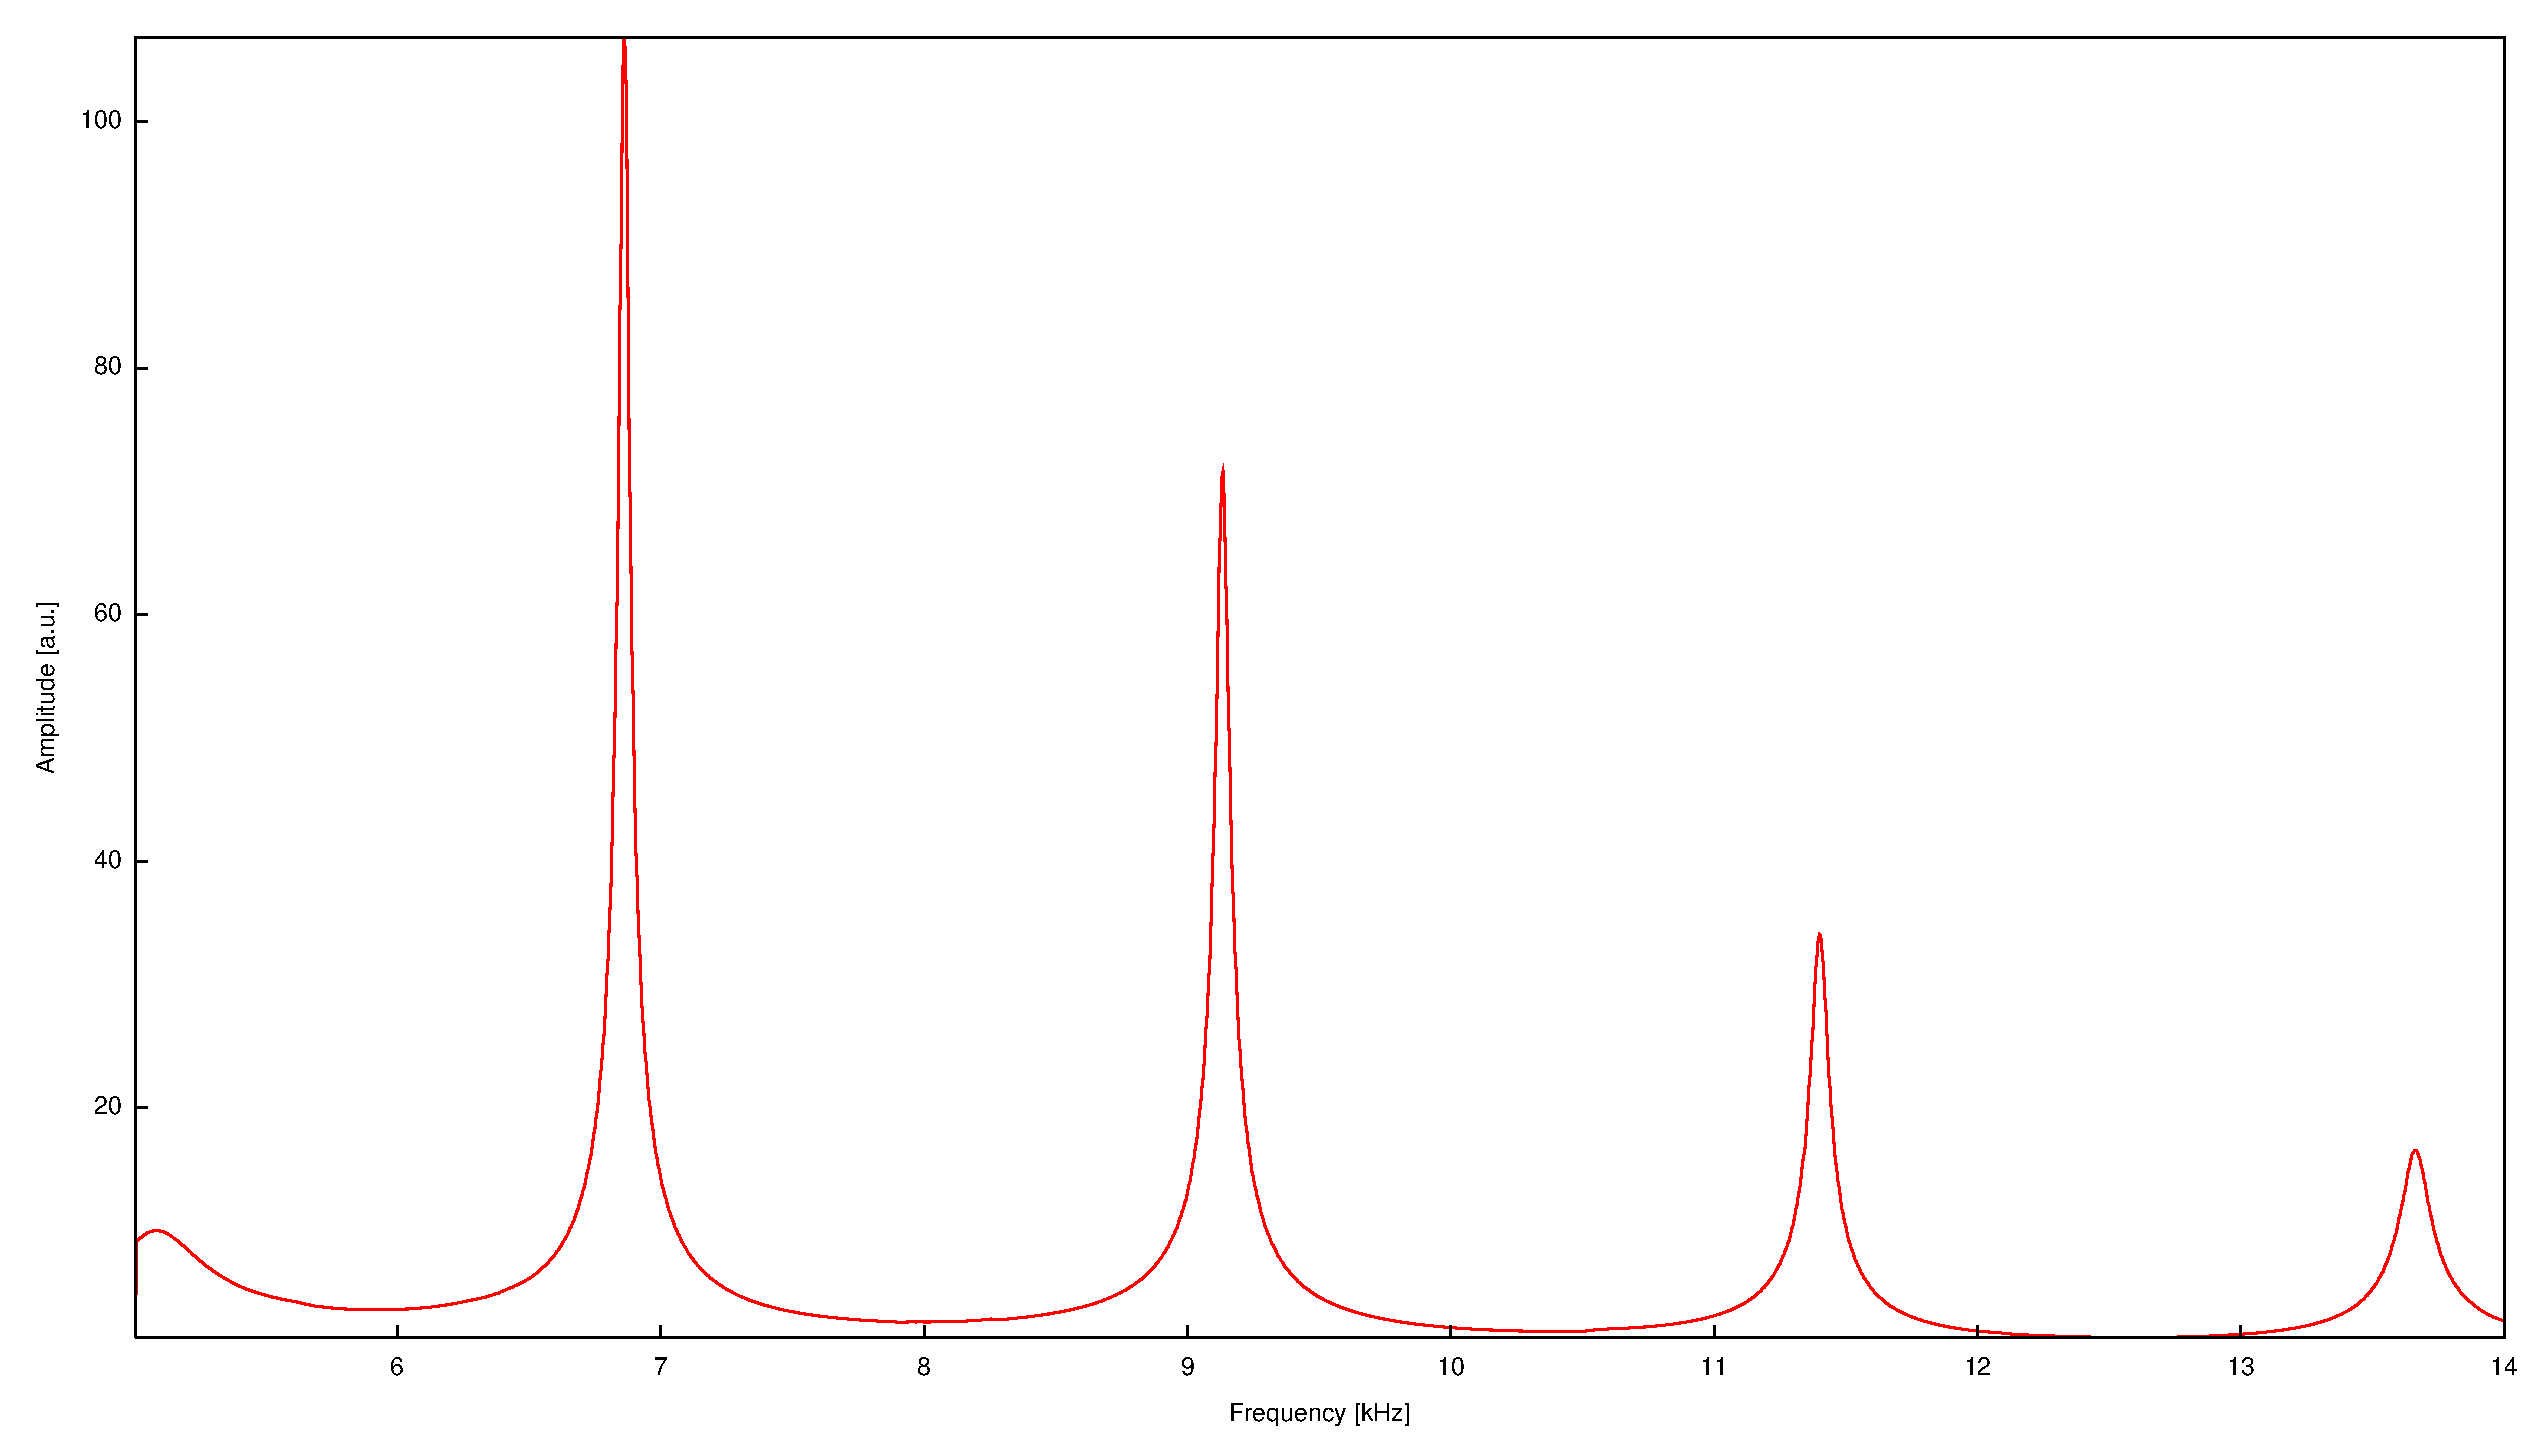
\includegraphics[scale=0.35]{FP-V23data/4.1_75mm.eps}
\caption{Spektrum von einer $\SI{75}{\milli\meter}$-Röhre.}
\label{fig:Spek4_1}
\end{figure}
\begin{table}
\centering
\caption{Mittlerer Abstand der Peaks}
\label{tab:mu}
	\sisetup{table-format=1.2}
	\begin{tabular}{S[table-format=3.0]S[table-format=4.0]@{${}\pm{}$}S[table-format=1.0]}
		\toprule
		{$L/\si{\milli\meter}$} & \multicolumn{2}{c}{$\Delta f/\si{\hertz}$} \\
		\midrule
		 75  & 2268 & 4 \\
		 150 & 1139 & 3 \\
		 225 & 763  & 2 \\
		 300 & 574 & 2 \\
		 375 & 459 & 2 \\
		 450 & 383 & 1 \\
		 525 & 327 & 1 \\
		 600 & 287 & 1 \\
		\bottomrule
	\end{tabular}

\end{table}
\begin{figure}
\centering
\includegraphics[scale=0.35]{build/4.1.pdf}
\caption{$\Delta f$ aufgetragen gegen $\frac{1}{L}$ zur Bestimmung der Schallgeschwindigkeit $c$.}
\label{fig:Df_L}
\end{figure}
\begin{figure}
\centering
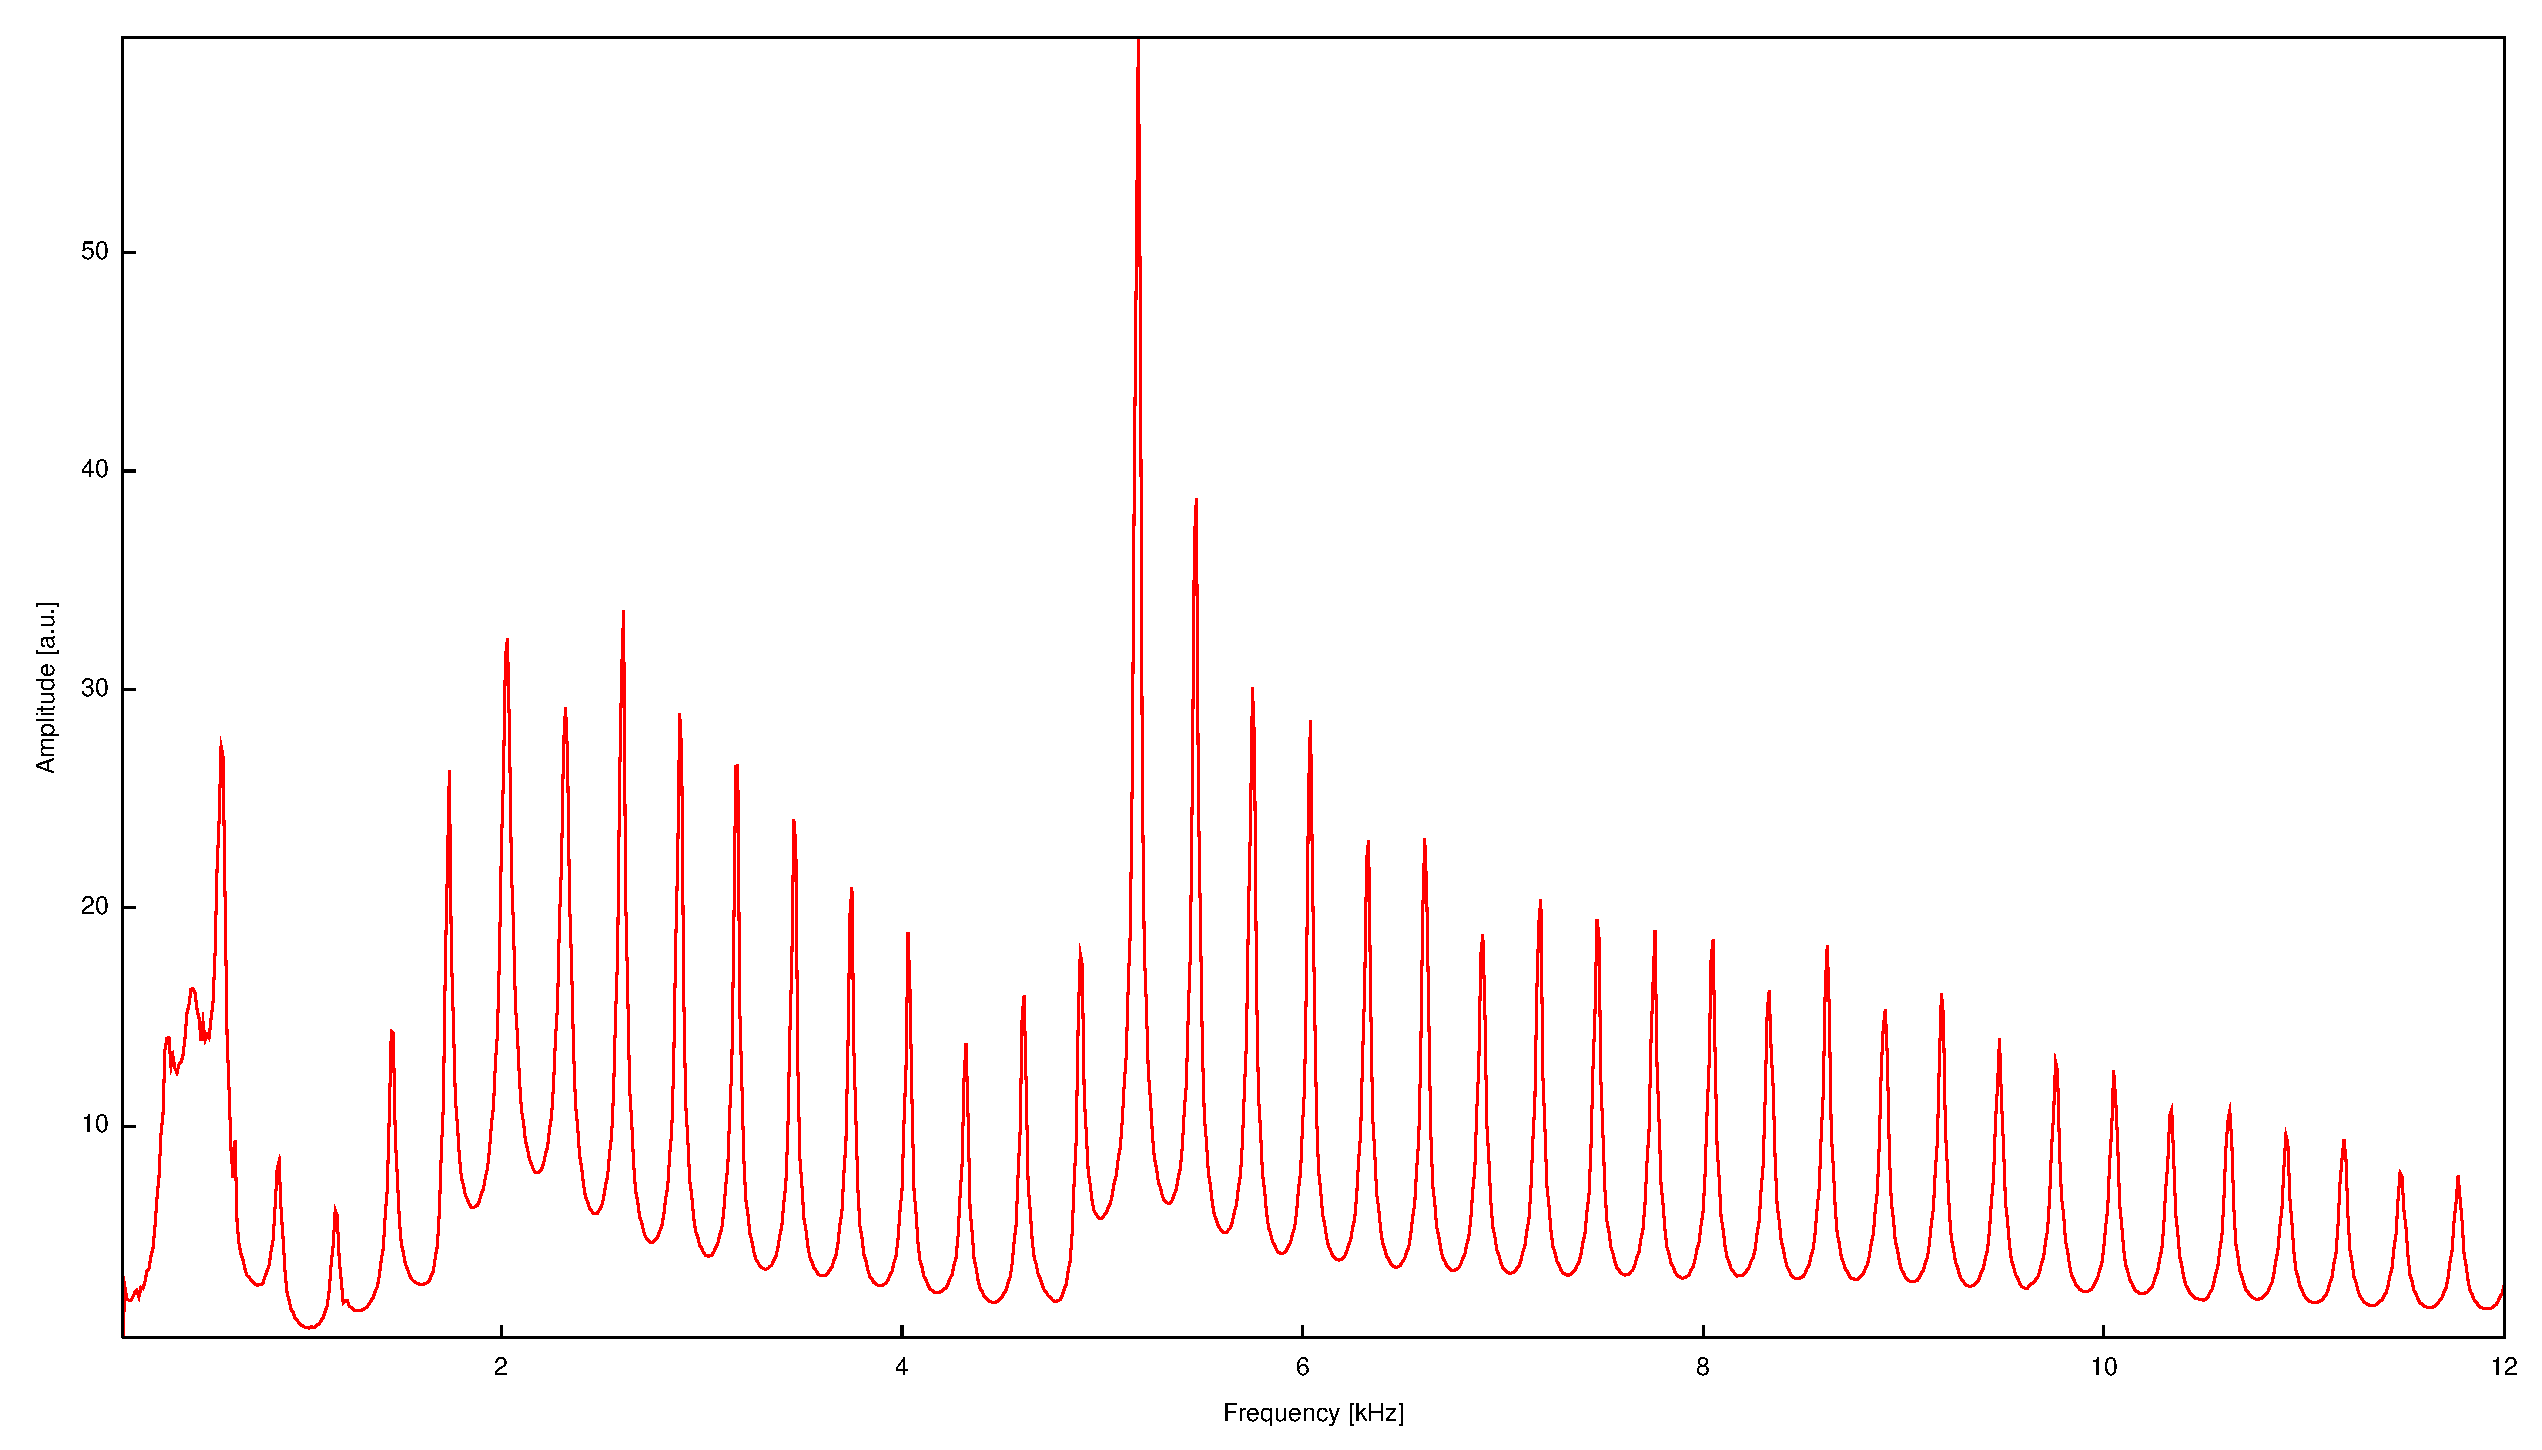
\includegraphics[scale=0.35]{FP-V23data/4.2_600mm.eps}
\caption{Spektrum von zwölf $\SI{50}{\milli\meter}$-Röhren.}
\label{fig:12_50}
\end{figure}
\begin{figure}
\centering
\includegraphics[scale=0.35]{build/4.2.pdf}
\caption{Dispersionsrelation $\omega(k)$ von zwölf $\SI{50}{\milli\meter}$-Röhren}
\label{fig:w_k}
\end{figure}
%\begin{figure}
%\centering
%\includegraphics[scale=0.35]{build/4.3_10mm.pdf}
%\caption{•}
%\label{fig:w_k_1}
%\end{figure}
%\begin{figure}
%\centering
%\includegraphics[scale=0.35]{build/4.3_13mm.pdf}
%\caption{•}
%\label{fig:w_k_2}
%\end{figure}
%\begin{figure}
%\centering
%\includegraphics[scale=0.35]{build/4.3_16mm.pdf}
%\caption{•}
%\label{fig:w_k_3}
%\end{figure}
\begin{figure}
\centering
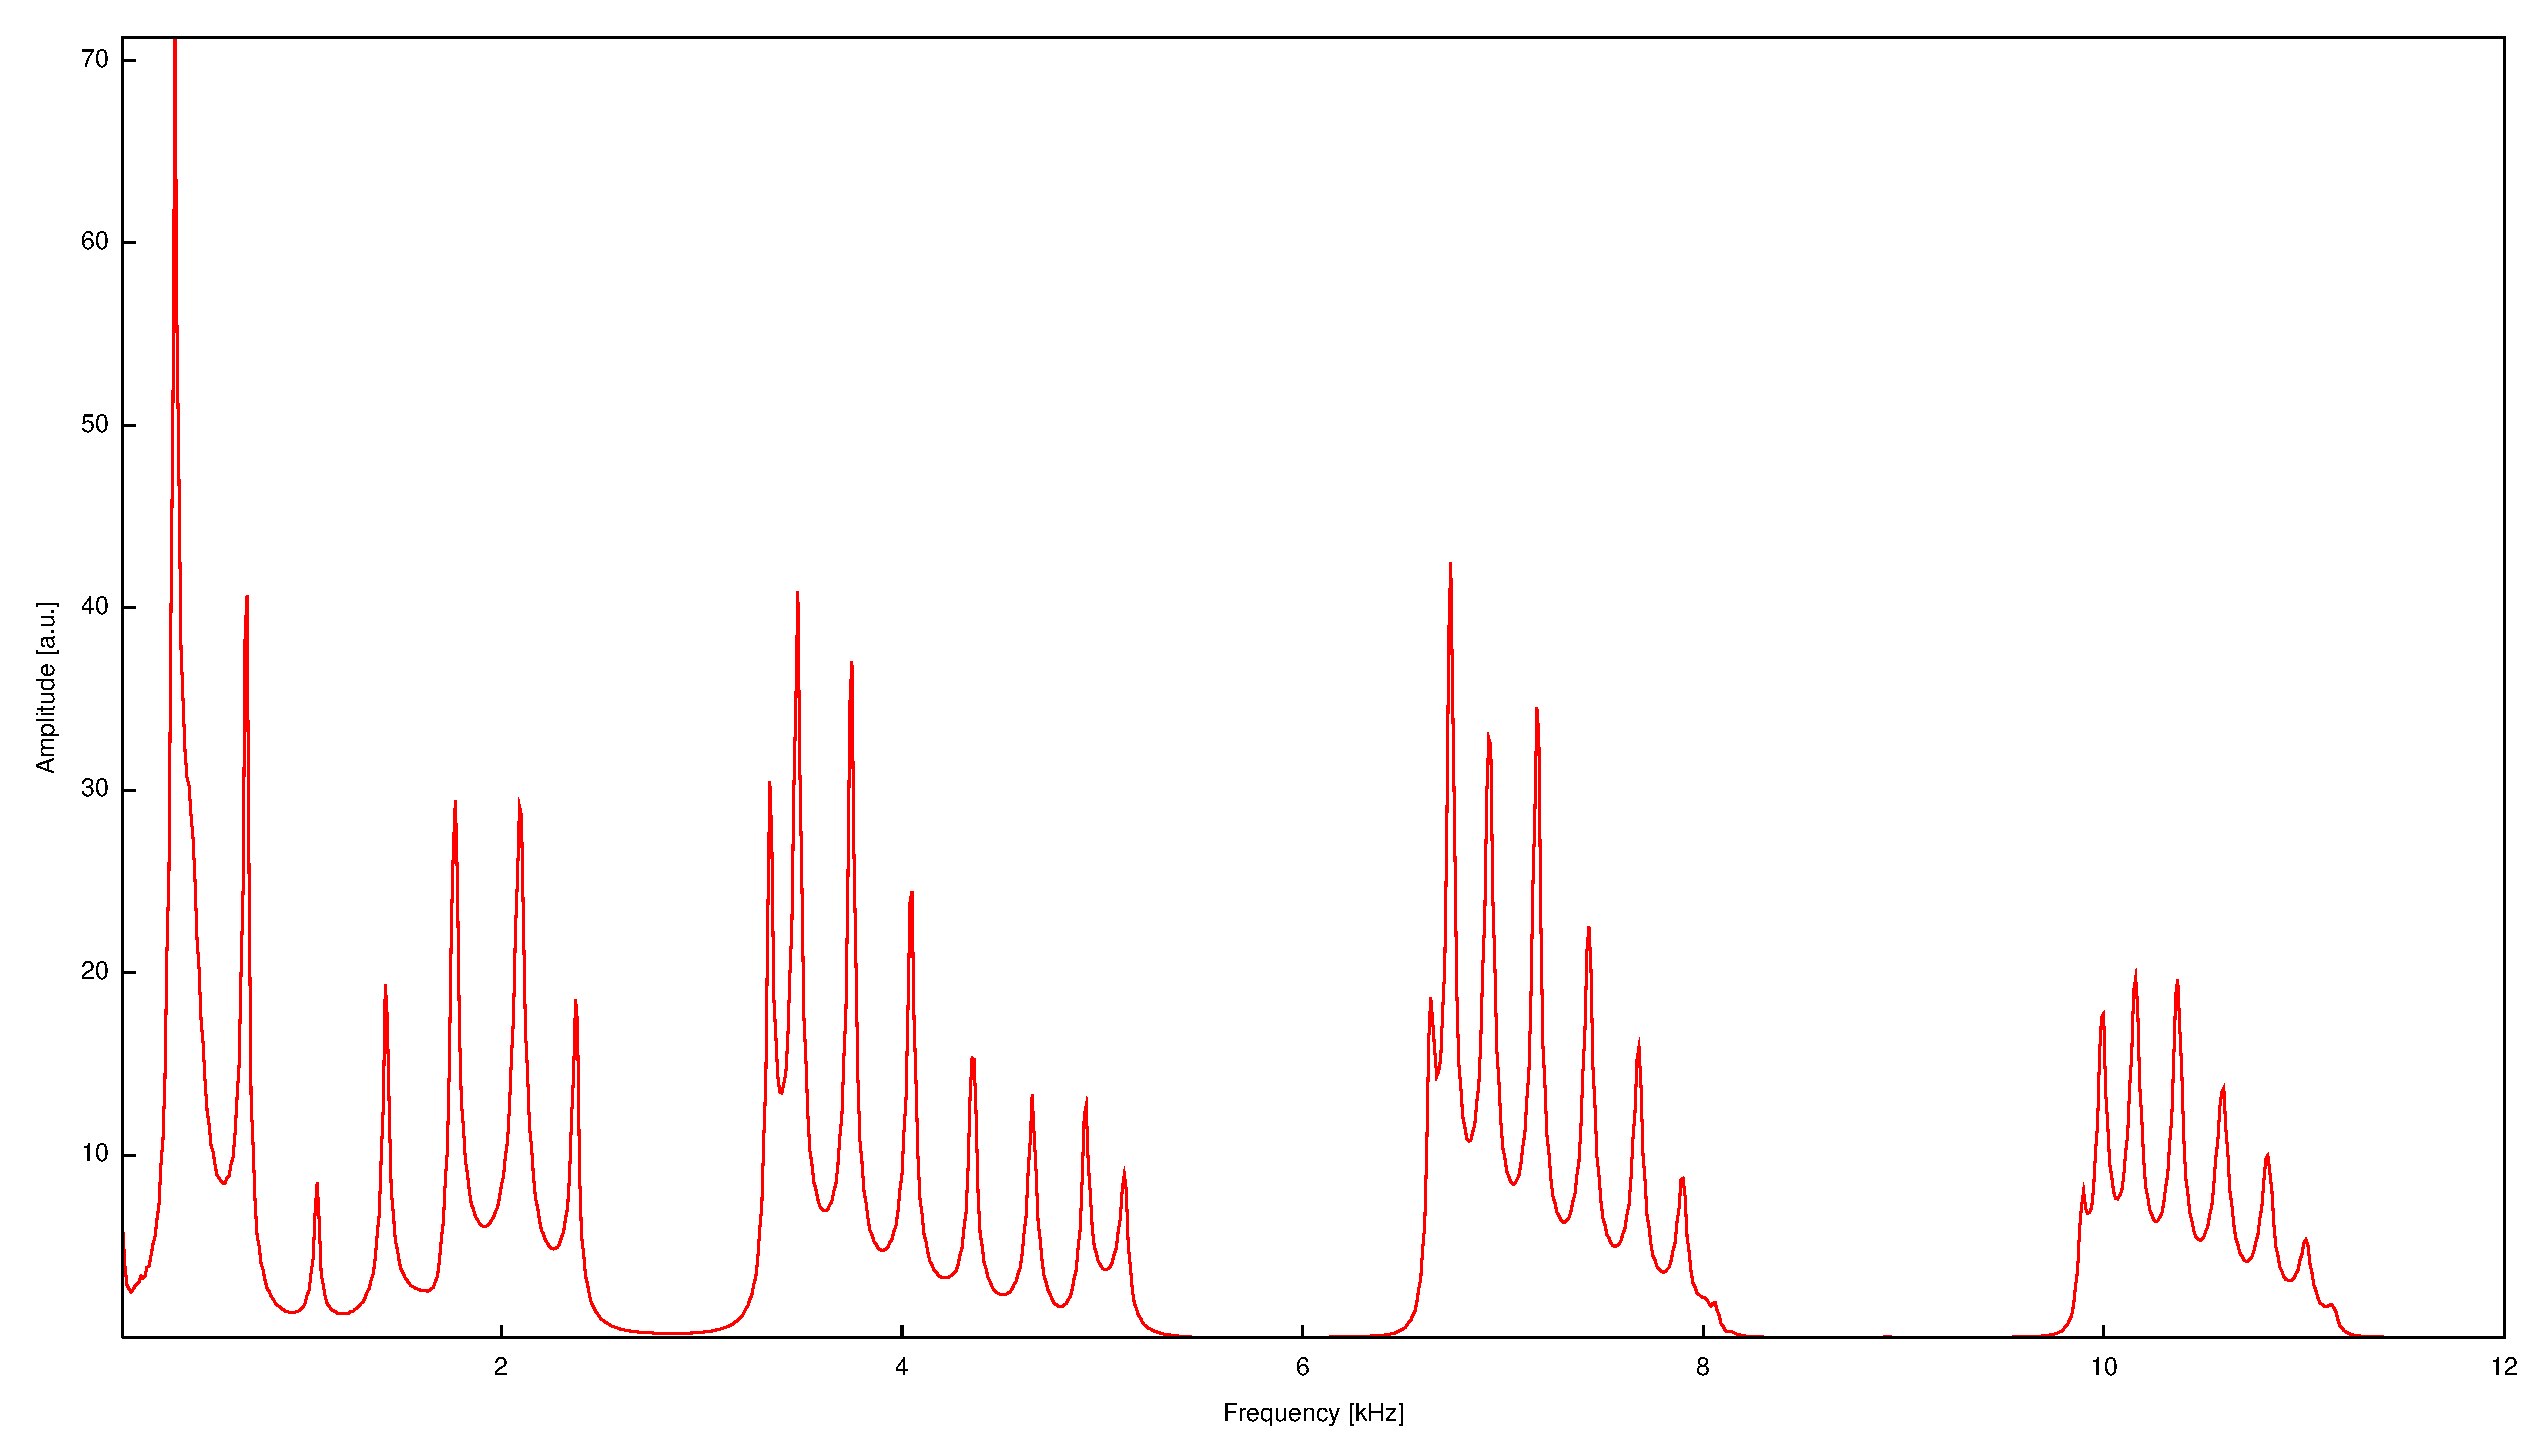
\includegraphics[scale=0.35]{FP-V23data/4.3_400mm_16mm.eps}
\caption{Spektrum von acht über $\SI{16}{\milli\meter}$-Irisse gekoppelten $\SI{50}{\milli\meter}$-Röhren}
\label{fig:8_50_16}
\end{figure}
\begin{figure}
\centering
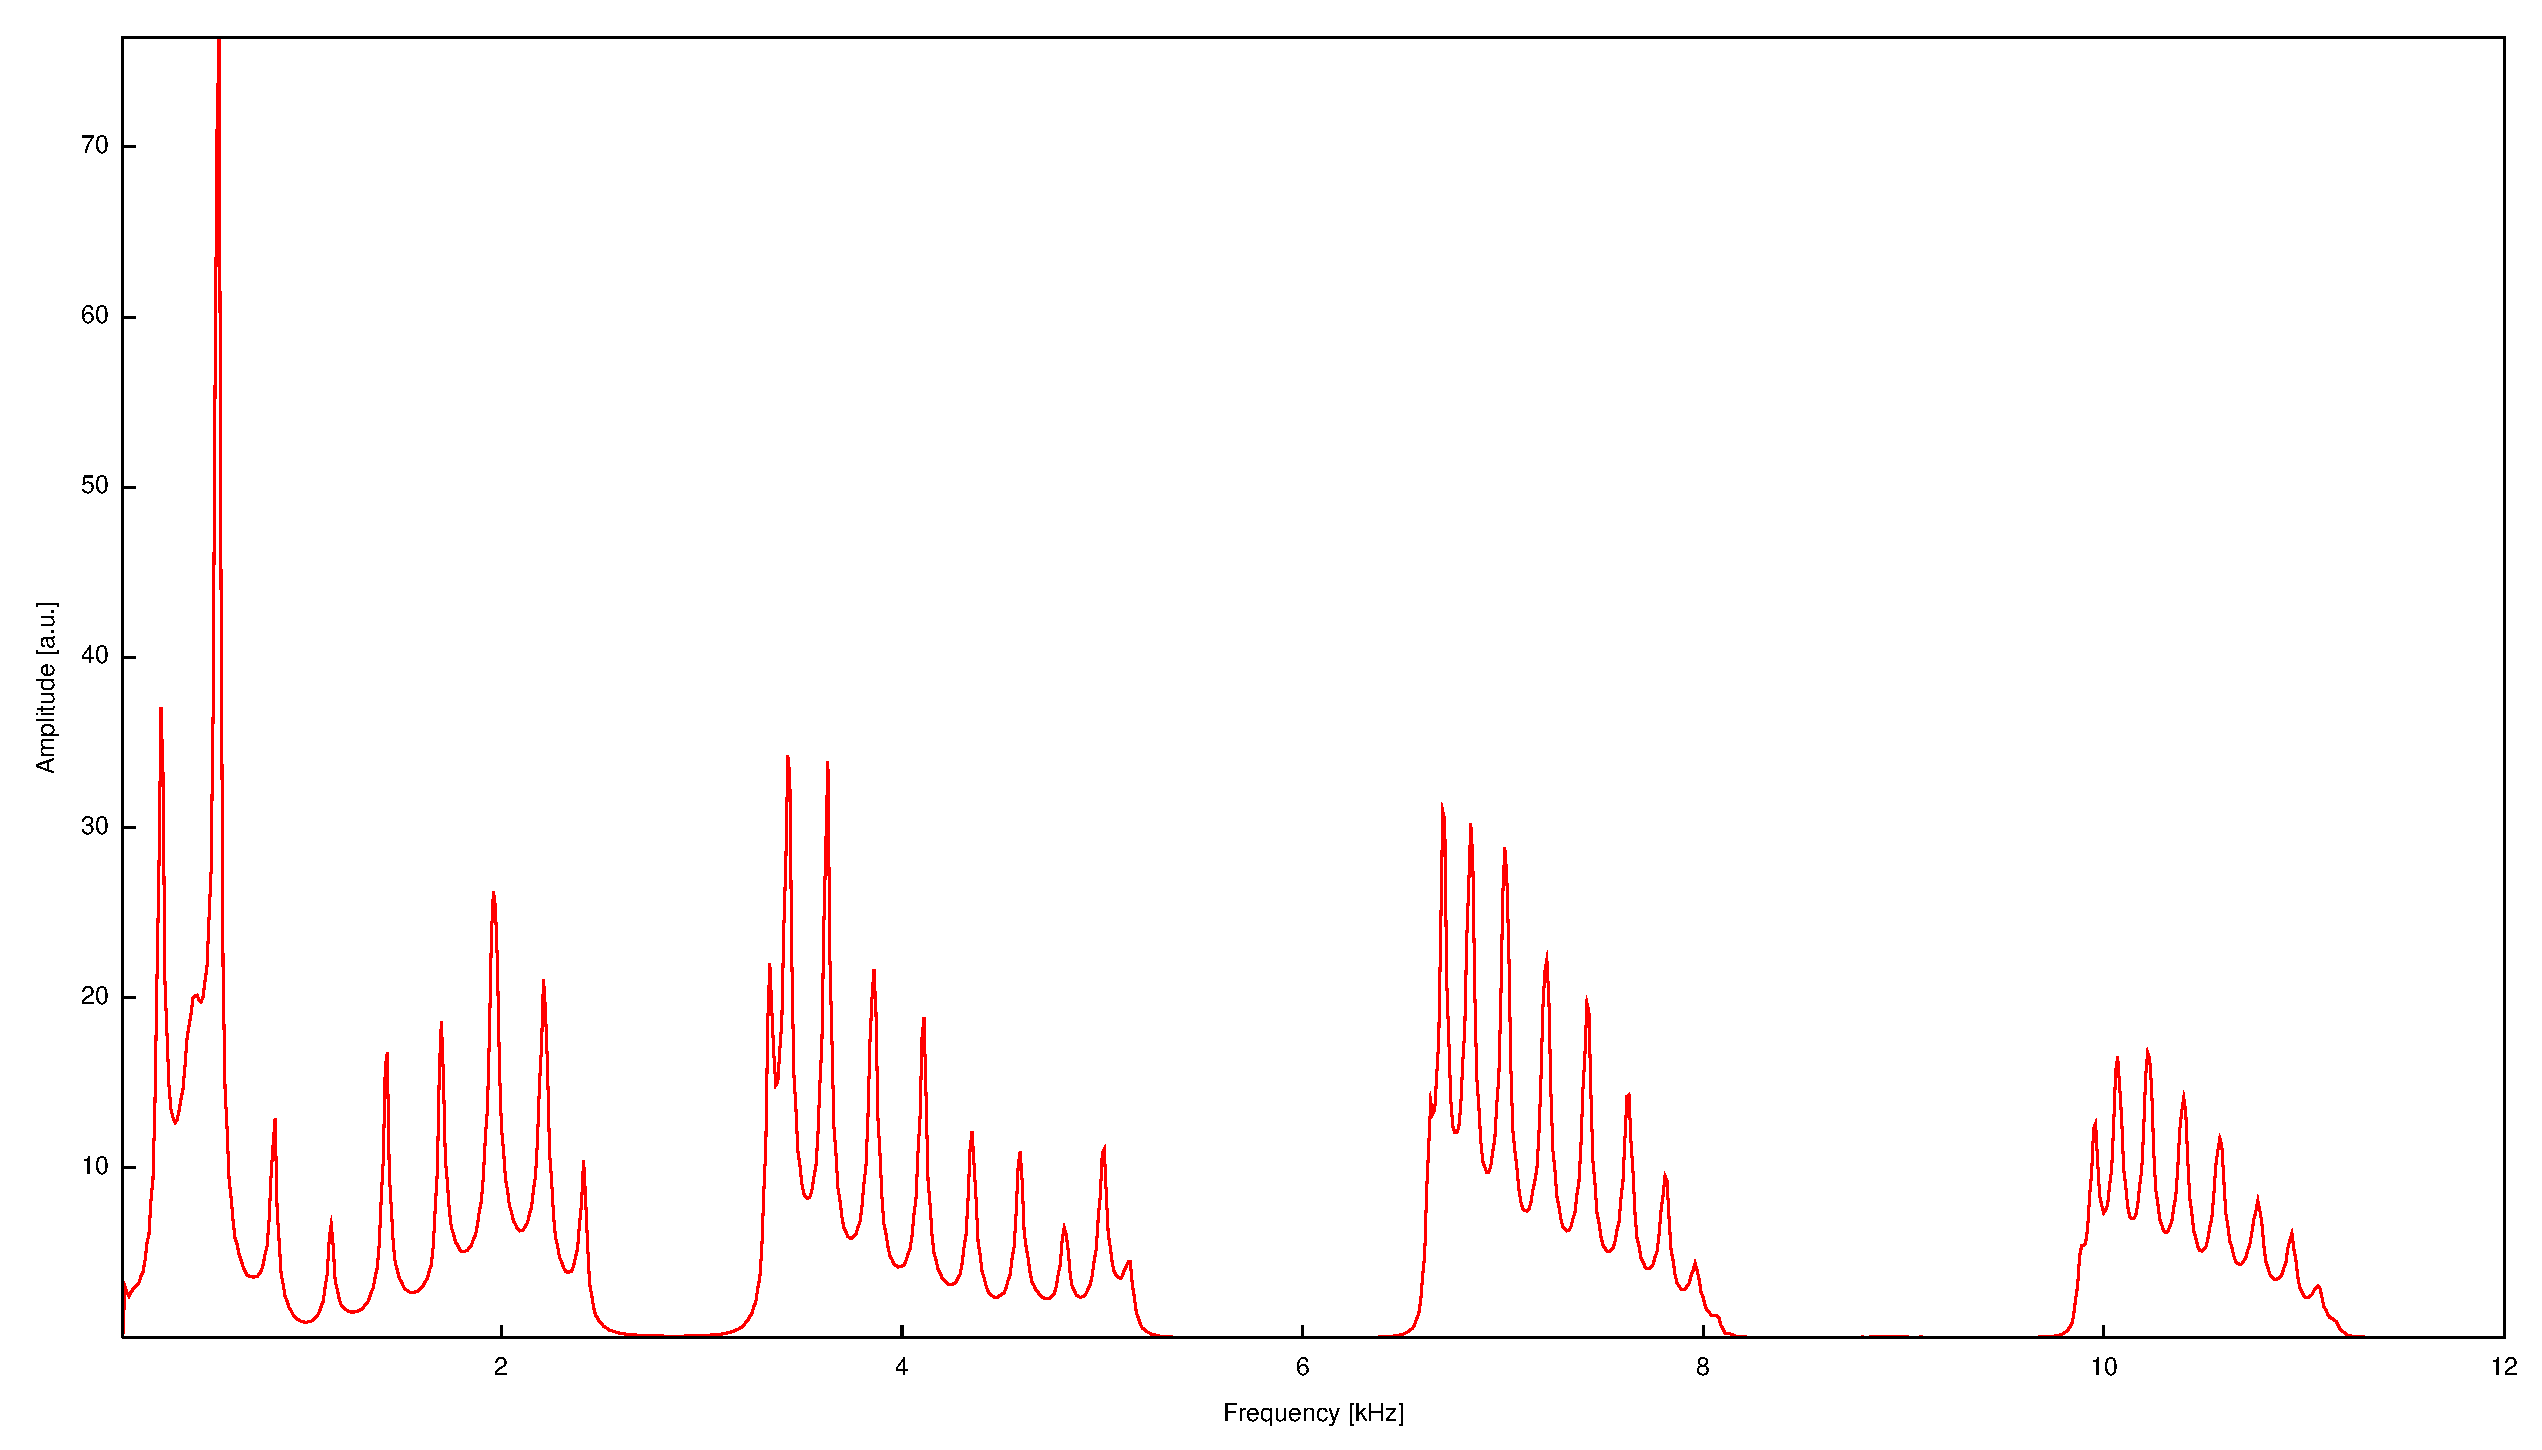
\includegraphics[scale=0.35]{FP-V23data/4.4_500mm_16mm.eps}
\caption{Spektrum von zehn über $\SI{16}{\milli\meter}$-Irisse gekoppelten $\SI{50}{\milli\meter}$-Röhren}
\label{fig:10_50_16}
\end{figure}
\begin{figure}
\centering
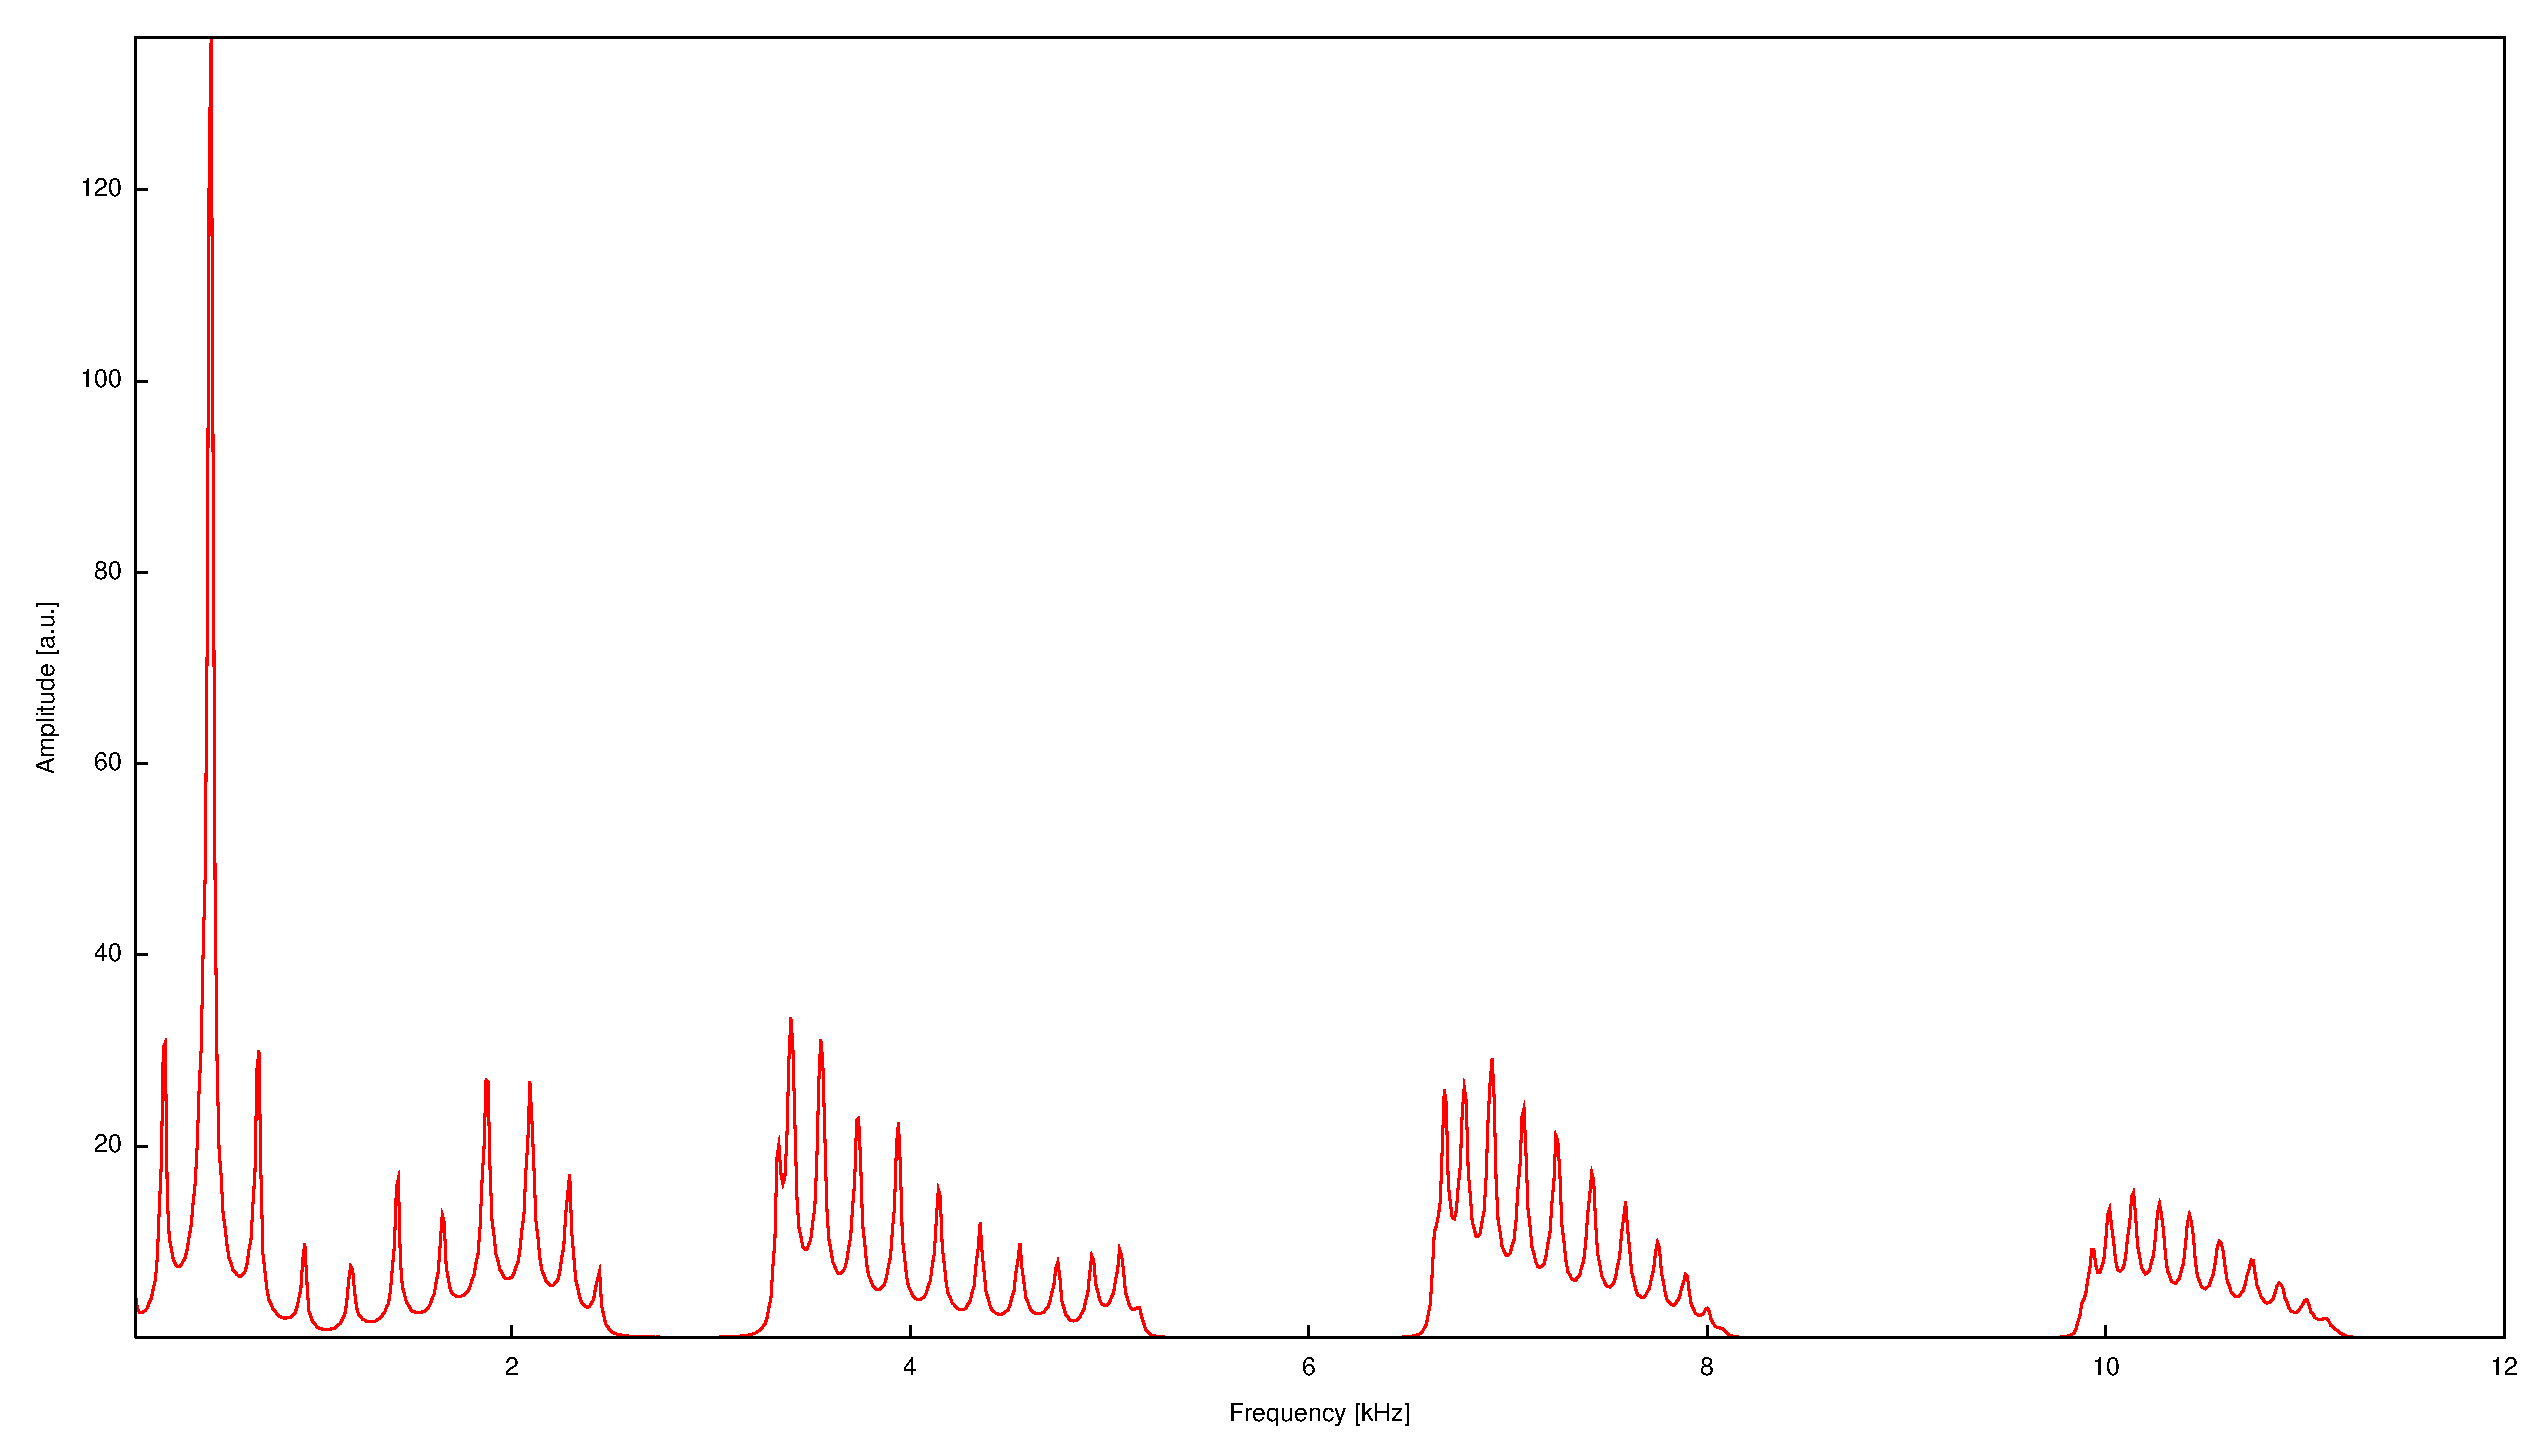
\includegraphics[scale=0.35]{FP-V23data/4.4_600mm_16mm.eps}
\caption{Spektrum von zwölf über $\SI{16}{\milli\meter}$-Irisse gekoppelten $\SI{50}{\milli\meter}$-Röhren}
\label{fig:12_50_16}
\end{figure}
\begin{figure}
\centering
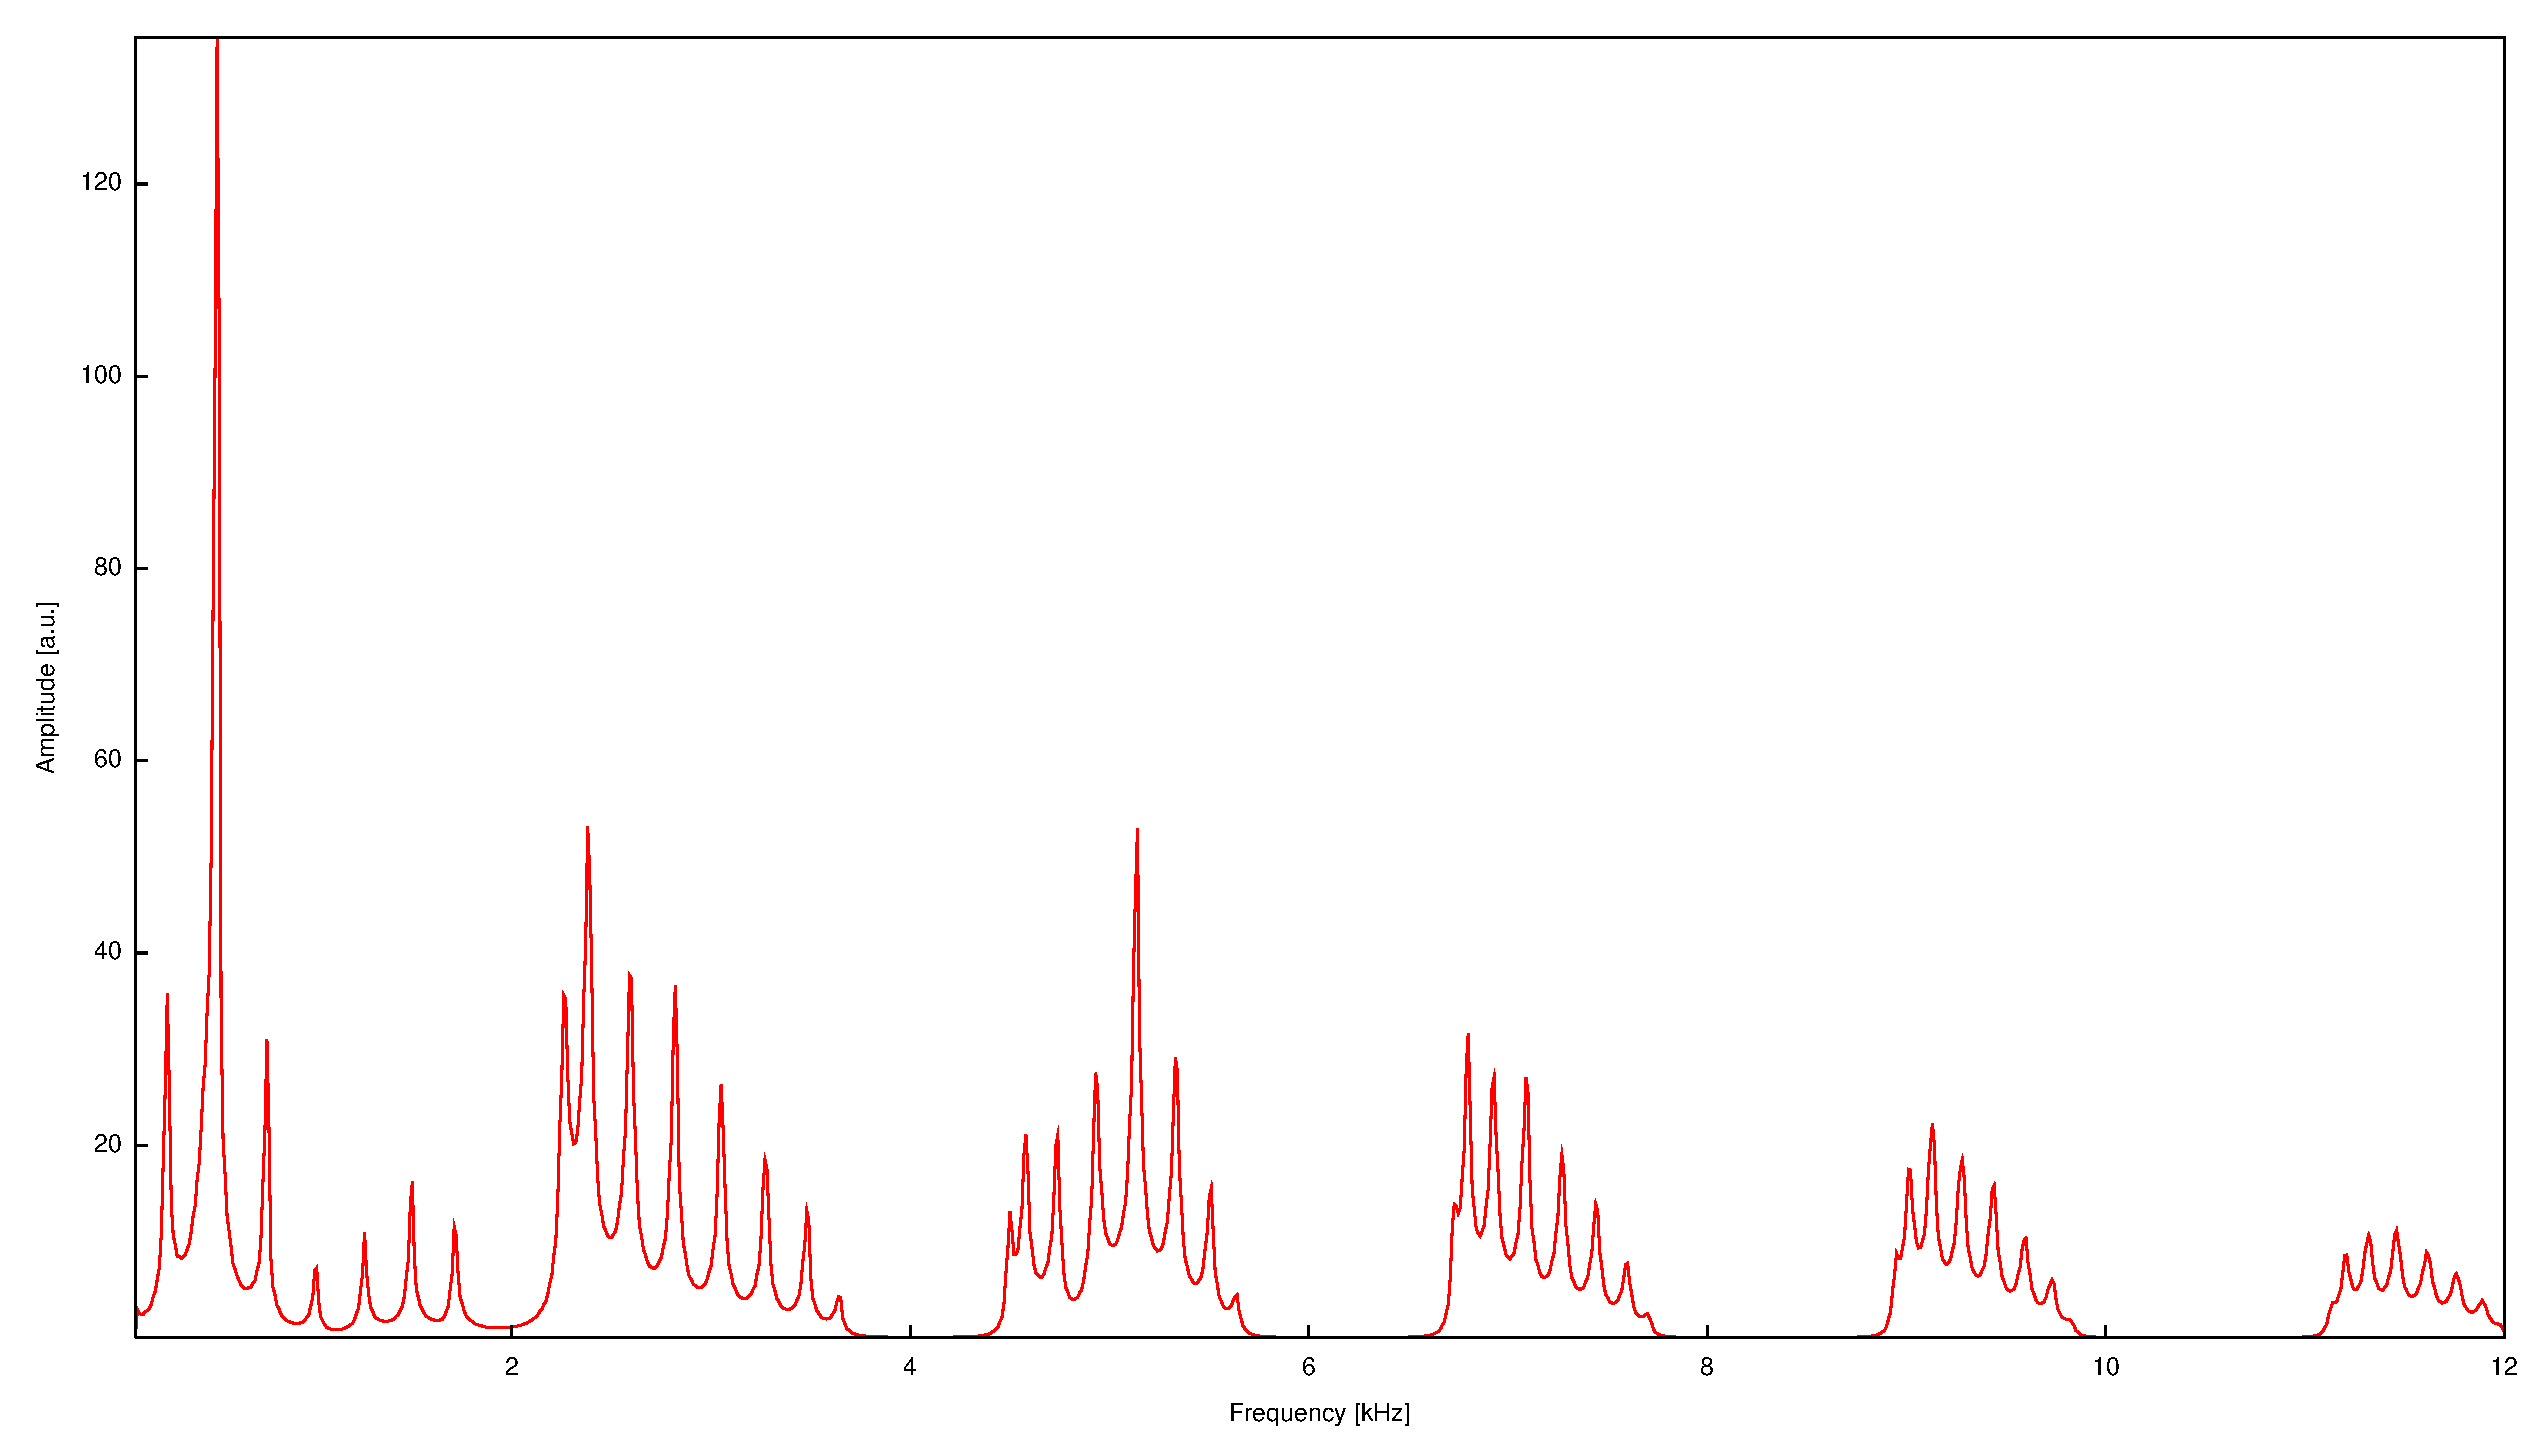
\includegraphics[scale=0.35]{FP-V23data/4.5_600mm_16mm.eps}
\caption{Spektrum von acht über $\SI{16}{\milli\meter}$-Irisse gekoppelten $\SI{75}{\milli\meter}$-Röhren}
\label{fig:8_75_16}
\end{figure}
\subsection{Atom-Molekül-Kette und Fehlstellen}
In Abbildung \ref{fig:50mm} ist das Spektrum einer $\SI{50}{\milli\meter}$-Röhre von $\SI{100}{\hertz}$ bis $\SI{22000}{\hertz}$ zu sehen. Bis $f\approx\SI{15000}{\hertz}$
sind die Peaks äquidistante longitudinale Moden. Für höhere Frequenzen sind die Abstände nicht mehr gleichmäßig und die Amplituden der Peaks wesentlich geringer. Sie beschreiben die transversalen Moden der Schallwelle in der Röhre.\\
In Abbildung \ref{fig:75mm} ist dasselbe Spektrum für eine $\SI{75}{\milli\meter}$-Röhre aufgenommen. Auch hier sind die longitudinalen Moden durch äquidistante Peaks bis etwa $\SI{15000}{\hertz}$ zu erkennen.\\
In Abbildung \ref{fig:50_10_50} ist das Spektrum von $\SI{100}{\hertz}$ bis $\SI{22000}{\hertz}$ einer Einheitszelle bestehend aus zwei über eine $\SI{10}{\milli\meter}$-Iris gekoppelten $\SI{50}{\milli\meter}$-Röhren zu sehen. Dieselbe Messung für eine $\SI{16}{\milli\meter}$-Kopplung ist in Abbildung \ref{fig:50_16_50} zu sehen. Es zeigt sich, dass die Breite der Bänder bei größerer Kopplung steigt während die Höhe der Peaks abnimmt. Auch ist bei größerem Innendurchmesser der Iris ein stärkerer Untergrund zu beobachten\\
%4.9?
In Abbildung \ref{fig:12_50_13_16} ist das Spektrum einer Folge von zwölf $\SI{50}{\milli\meter}$-Röhren, die abwechselnd über $\SI{13}{\milli\meter}$- und über $\SI{16}{\milli\meter}$-Irisse gekoppelt sind. Der Vergleich mit Abbildung \ref{fig:12_50_16} zeigt, dass sich bei alternierender Kopplung innerhalb der Bänder eine Substruktur bildet, die Anzahl der Peaks jedoch konstant bleibt.



%◘♦☻♥◘○☺♠◘

	
\section{Diskussion}
\label{sec:Diskussion}

\begin{table}
	\centering
	\caption{Die in der Auswertung bestimmten Werte mit den zugehörigen Referenzwerten und Abweichungen.}
	\label{tab:Ergebnisse}
	\sisetup{table-format=1.2}
	\begin{tabular}{c ccc}
		\toprule
		{Wert}&{gemessen}&{Referenzwert\cite{cAcryl},\cite{alphaAcryl}}&{Abweichung} \\
		\midrule
		$l_.{Tiefenmessung}$ & \SI{120.04}\,\si{\milli\meter} & \SI{120.5}\,\si{\milli\meter} & \SI{-0.4}\,\si{\percent} \\
		$c_\text{1}$ & \SI{2708\pm17}\,\si{\meter\per\second} & \SI{2730}\,\si{\meter\per\second} & \SI{-0.8}\,\si{\percent} \\
		$c_\text{2}$ & \SI{2700\pm120}\,\si{\meter\per\second} & \SI{2730}\,\si{\meter\per\second} & \SI{-1.1}\,\si{\percent} \\
		$\alpha$ & \SI{61\pm17}\,\si{\per\meter} & \SI{57\pm2}\,\si{\per\meter} & \SI{7}\,\si{\percent} \\
		$\alpha_{I1}$ & \SI{8\pm2}\,\si{\per\meter} & \SI{57\pm3}\,\si{\per\meter} & \SI{-86}\,\si{\percent} \\
		$\alpha_{I2}$ & \SI{61\pm2}\,\si{\per\meter} & \SI{57\pm2}\,\si{\per\meter} & \SI{7}\,\si{\percent} \\
		$D_{1,1}$ & \SI{6.0}\,\si{\milli\meter} & \SI{6.0}\,\si{\milli\meter} & \SI{0}\,\si{\percent} \\
		$D_{1,2}$ & \SI{9.8}\,\si{\milli\meter} & \SI{9.8}\,\si{\milli\meter} & \SI{0}\,\si{\percent} \\
		$D_{2,1}$ & \SI{6.1}\,\si{\milli\meter} & \SI{6.0}\,\si{\milli\meter} & \SI{1.7}\,\si{\percent} \\
		$D_{2,2}$ & \SI{9.8}\,\si{\milli\meter} & \SI{9.8}\,\si{\milli\meter} & \SI{0}\,\si{\percent} \\
		$A_1$ & \SI{7.33}\,\si{\milli\meter} & - & - \\
		$A_2$ & \SI{4.09}\,\si{\milli\meter} & - & - \\
		$A_3$ & \SI{8.90}\,\si{\milli\meter} & - & - \\
		$A_4$ & \SI{35.3}\,\si{\milli\meter} & - & - \\
		\bottomrule
	\end{tabular}

	\label{tab:Ergebnisse}
\end{table}

\noindent In Tabelle \ref{tab:Ergebnisse} ist zu erkennen, dass die bestimmten Geschwindigkeiten $c_1$ und $c_2$ nah am Literaturwert liegen. Dabei ist die Abweichung, sowie der relative Fehler beim Durchschallungs-Verfahren größer als bei dem Impuls-Echo-Verfahren. Dies ist durch die halb so lange Strecke zu erklären, da Abweichungen in der Zeitmessung bei geringerer Zeit eine größere Rolle spielen. Die bei der Tiefenmessung bestimmte Länge des Zylinders stimmt mit der durch die Schieblehre bestimmten Länge überein.\\
Bei der Bestimmung des Dämpfungskonstanten $\alpha$ sind die schlechten Messwerte auffallend. Diese sind wahrscheinlich durch eine falsche Einstellung des Messgerätes zustande gekommen. In Abbildung \ref{fig:Daempfung} sind zwei mögliche Interpretationen der Messergebnisse zu sehen. Werden die Ergebnisse dieser mit dem Literaturwert von $\SI{57(3)}{\per\metre}$ verglichen, scheint die zweite Interpretation mit $\alpha_2=\SI{61(2)}{\per\metre}$ die naheliegende zu sein, obwohl mehr Punkte auf der ersten Ausgleichsgeraden liegen. Dies lässt vermuten, dass die Messung im niedrigen Bereich zu starke Spannungen geliefert hat, was möglicherweise auf eine falsche Einstellung der Verstärkung hindeutet.\\
Die Messung der Dicken der Acrylplatten ist hingegen sehr genau, da hier die berechneten Werte aus dem Cepstrum und dem Spektrum kaum von den gemessenen Werten mit der Schieblehre abweichen. Dabei werden die Werte für die Zeitdifferenzen für das Cepstrum aus Abbildung \ref{fig:Cepstrum} entnommen. Die Abstände für das Auge scheinen ebenfalls in der richtigen Größenordnung zu liegen, sind jedoch ohne Standardwerte nicht weiter zu überprüfen.     
	\newpage
	\printbibliography[title=Literatur]
\end{document}